Los capítulos anteriores han descrito tres técnicas base de generación de lenguaje natural ---gramática formal, embeddings semánticos y modelos de lenguaje grandes--- y tres hibridaciones que las combinan. Cada una ha sido evaluada individualmente sobre su propio corpus. Este capítulo las confronta sobre un mismo conjunto de datos mediante un pipeline de evaluación automatizado que aplica métricas con referencia, sin referencia y específicas de CAA, complementadas con tests de significancia estadística y visualizaciones comparativas. El objetivo no es proclamar un ganador, sino cartografiar las fortalezas, debilidades y compromisos de cada enfoque.

\section{Metodología de la evaluación}
\label{sec:eval-metodologia}

La comparación rigurosa de seis motores de generación requiere un protocolo que garantice la equidad de condiciones. El pipeline de evaluación opera en cinco pasos secuenciales:

\begin{enumerate}
    \item \textit{Unificación del dataset}: los tres conjuntos de datos de las técnicas base ---cada uno con formato y campos ligeramente diferentes--- se normalizan a un formato canónico y se calcula su intersección por identificador. El resultado son 428 casos comunes que constituyen el corpus de evaluación unificado.
    \item \textit{Generación}: cada uno de los seis motores procesa los 428 casos y produce una oración de salida por caso. Los resultados se almacenan en caché para garantizar reproducibilidad. De los 428 casos, solo 115 disponen de salidas cacheadas del LLM ---los que se evaluaron originalmente con llamadas reales a la API de OpenAI---; los 313 restantes no tienen salida LLM, lo que afecta a las métricas de ese motor y, por extensión, a las comparaciones estadísticas.
    \item \textit{Cálculo de métricas}: para cada par (predicción, referencia) se calculan las métricas descritas en la Sección~\ref{sec:metricas}. En total se obtienen 17 valores por caso y motor.
    \item \textit{Análisis estadístico}: se aplican tests de significancia no paramétricos ---Friedman como test ómnibus, Wilcoxon signed-rank por pares con correcciones de Bonferroni y Holm-Bonferroni, y bootstrap pareado para intervalos de confianza--- sobre las distribuciones de métricas de los seis motores.
    \item \textit{Generación de informes}: tablas comparativas, gráficas de distribución y plantillas para evaluación humana.
\end{enumerate}

Una observación fundamental para interpretar los resultados: los motores de gramática formal y embeddings semánticos obtienen scores perfectos o casi perfectos en las métricas de coincidencia porque las oraciones de referencia del dataset fueron generadas originalmente por estos motores. La referencia \textit{es} su salida, de modo que la coincidencia es trivial por diseño. Estos valores no indican superioridad sino que constituyen el techo teórico del dataset ---el máximo que cualquier motor podría alcanzar si reprodujera exactamente las mismas formulaciones.

\section{Resultados globales}
\label{sec:eval-resultados}

Las Tablas~\ref{tab:eval-referencia} y~\ref{tab:eval-sin-referencia} resumen el rendimiento de los seis motores. Cada celda muestra la media $\pm$ desviación estándar sobre los 428 casos.

\begin{table}[H]
\centering
\small
\begin{tabular}{l c c c c c c}
\hline
 & \multicolumn{2}{c}{Técnicas base} & & \multicolumn{3}{c}{Hibridaciones} \\
\cline{2-3} \cline{5-7}
Métrica & Gramática & LLM & & Híbrido 1 & Híbrido 2 & Híbrido 3 \\
\hline
EM & 1,00 & 0,25 $\pm$ 0,43 & & 0,85 $\pm$ 0,36 & 0,86 $\pm$ 0,35 & 0,88 $\pm$ 0,32 \\
BLEU-1 & 1,00 & 0,26 $\pm$ 0,43 & & 0,94 $\pm$ 0,14 & 0,95 $\pm$ 0,13 & 0,96 $\pm$ 0,13 \\
BLEU-4 & 1,00 & 0,26 $\pm$ 0,43 & & 0,91 $\pm$ 0,22 & 0,92 $\pm$ 0,20 & 0,93 $\pm$ 0,21 \\
METEOR & 0,98 $\pm$ 0,02 & 0,25 $\pm$ 0,42 & & 0,92 $\pm$ 0,18 & 0,93 $\pm$ 0,16 & 0,93 $\pm$ 0,15 \\
chrF++ & 1,00 & 0,26 $\pm$ 0,43 & & 0,94 $\pm$ 0,14 & 0,95 $\pm$ 0,13 & 0,96 $\pm$ 0,12 \\
ROUGE-L $F_1$ & 1,00 & 0,26 $\pm$ 0,44 & & 0,96 $\pm$ 0,11 & 0,96 $\pm$ 0,10 & 0,97 $\pm$ 0,10 \\
BERTScore $F_1$ & 1,00 & 0,80 $\pm$ 0,12 & & 0,99 $\pm$ 0,04 & 0,99 $\pm$ 0,03 & 0,99 $\pm$ 0,03 \\
\hline
\end{tabular}
\caption{Métricas con referencia por motor (media $\pm$ desviación estándar, $n=428$). La gramática formal y los embeddings semánticos producen salidas idénticas en 426 de 428 casos (99,5\%), por lo que se presentan en una sola columna. Los valores del LLM ($\sim$0,25) reflejan que solo 115 de los 428 casos disponen de salida cacheada; los 313 restantes se tratan como predicciones vacías. Los valores de Gramática sin desviación estándar indican $\sigma = 0$.}
\label{tab:eval-referencia}
\end{table}

\begin{table}[H]
\centering
\small
\begin{tabular}{l c c c c c c}
\hline
 & \multicolumn{2}{c}{Técnicas base} & & \multicolumn{3}{c}{Hibridaciones} \\
\cline{2-3} \cline{5-7}
Métrica & Gramática & LLM & & Híbrido 1 & Híbrido 2 & Híbrido 3 \\
\hline
Perplejidad & 161 & ---$^{*}$ & & 100 & 102 & 151 \\
Pseudo-perpl. & 33 & 4$^{*}$ & & 18 & 18 & 32 \\
Cobertura & 0,972 & 0,264 & & 0,983 & 0,980 & 0,986 \\
Fidelidad & 0,918 & 0,971 & & 0,936 & 0,934 & 0,933 \\
Latencia (ms) & 0,02 & 375 & & 811 & 915 & 4279 \\
Éxito & 1,000 & 0,269 & & 1,000 & 1,000 & 1,000 \\
\hline
\end{tabular}
\caption{Métricas sin referencia, métricas específicas de CAA y latencia por motor ($n=428$). Los valores de perplejidad y pseudo-perplejidad son medianas redondeadas. $^{*}$LLM: perplejidad GPT-2 no disponible (314 de 428 valores infinitos por salidas vacías); pseudo-perplejidad calculada solo sobre los 114 casos con salida finita. La tasa de éxito indica la proporción de casos que generaron salida no vacía.}
\label{tab:eval-sin-referencia}
\end{table}

La tabla de métricas con referencia revela un patrón condicionado por la cobertura parcial del LLM. Los motores base de gramática formal y embeddings semánticos alcanzan el techo del dataset por las razones ya expuestas. Los tres híbridos se sitúan en un rango alto: Exact Match del 85-88\%, BLEU-4 del 91-93\% y BERTScore de 0,99, lo que indica que en la mayoría de los casos reproducen formulaciones muy próximas a la referencia. El LLM, con valores de $\sim$0,25 en todas las métricas n-gramáticas, refleja su cobertura parcial: solo 115 de los 428 casos tienen salida cacheada, y los 313 restantes se evalúan como predicciones vacías. Estos scores no indican baja calidad lingüística del LLM ---sobre los 115 casos con salida, su rendimiento es alto, como se documenta en el capítulo correspondiente--- sino la ausencia de generación para los casos nuevos del dataset ampliado.

La tabla de métricas sin referencia completa el panorama. La cobertura de pictogramas converge en torno al 97-98\% para los cinco motores funcionales (gramática, embeddings y los tres híbridos), mientras que el LLM alcanza solo un 26,4\% por su cobertura parcial. La fidelidad de contenido muestra un patrón inverso: el LLM obtiene la más alta (0,971) porque sus 115 salidas tienden a ser fieles al input, mientras que los motores basados en gramática se sitúan en 0,918. La perplejidad revela que los híbridos 1 y 2 producen texto más natural que las técnicas base: medianas de 100 y 102 frente a 161 de la gramática. Hybrid3, con mediana de 151, se aproxima a la gramática en lugar de mejorarla, un resultado inesperado respecto a su diseño de ranking por perplejidad. La latencia mantiene un espectro amplio: desde los 0,02 ms de la gramática formal hasta los 4,3 segundos de Hybrid3.

\begin{figure}[H]
    \centering
    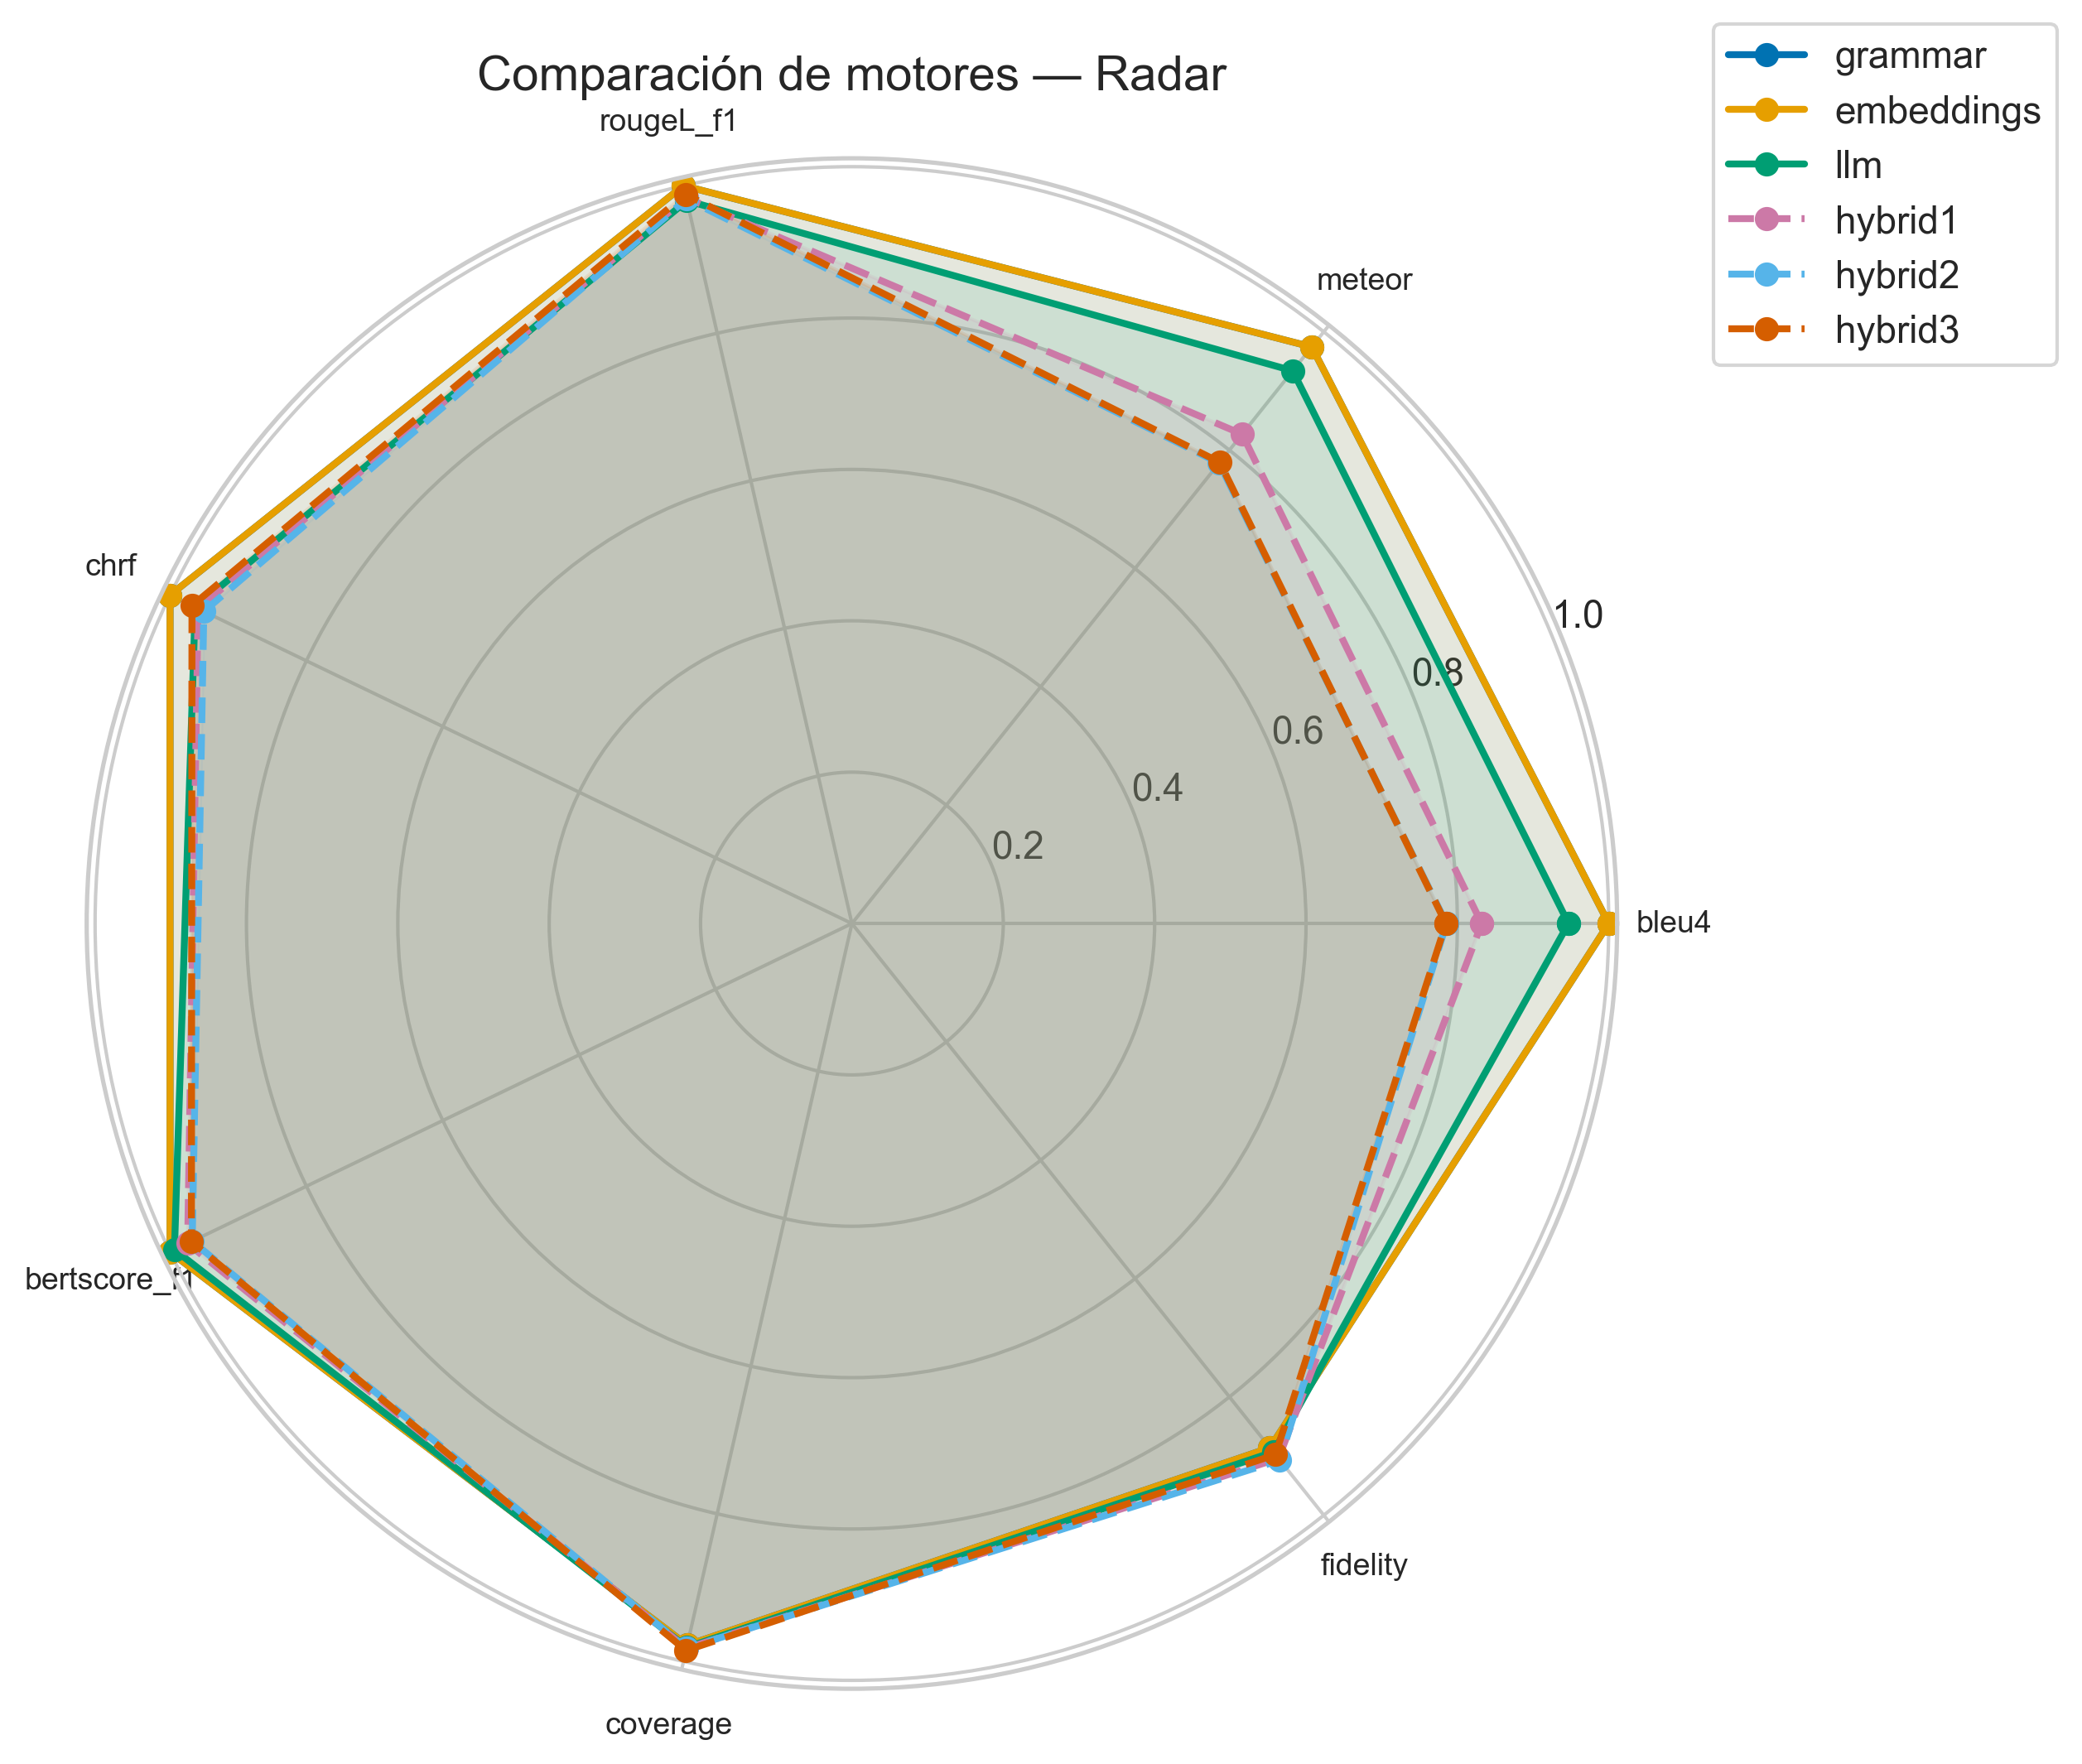
\includegraphics[width=0.85\textwidth]{figures/eval-radar.png}
    \caption{Perfil multimétrica de los seis motores. Líneas continuas para las técnicas base, discontinuas para las hibridaciones. Las técnicas base dominan las métricas de coincidencia (ejes superiores), mientras que los híbridos se aproximan en ROUGE-L, chrF++ y cobertura (ejes inferiores).}
    \label{fig:eval-radar}
\end{figure}

La Figura~\ref{fig:eval-radar} sintetiza visualmente este panorama. El perfil de la gramática formal y los embeddings forma un polígono que cubre prácticamente toda la superficie del radar. Los tres híbridos comparten un perfil ligeramente comprimido en los ejes de métricas n-gramáticas pero que se expande hacia los ejes de cobertura y fidelidad, donde convergen con las técnicas base. El LLM presenta el perfil más contraído por el efecto de su cobertura parcial, que arrastra todas las métricas de coincidencia hacia valores bajos.

\section{Significancia estadística}
\label{sec:eval-significancia}

Las diferencias numéricas entre motores solo son informativas si superan la variabilidad aleatoria del muestreo. Para verificarlo, se aplica un protocolo de tests no paramétricos ---elegidos porque las distribuciones de métricas de NLP no cumplen los supuestos de normalidad que requieren los tests paramétricos.

El test de Friedman actúa como test ómnibus: evalúa si existe al menos un motor significativamente diferente de los demás para cada métrica. Cuando Friedman rechaza la hipótesis nula, se procede a comparaciones por pares con el test de Wilcoxon signed-rank, que compara dos muestras relacionadas (los mismos 428 casos evaluados por dos motores diferentes). Con 6 motores existen $\binom{6}{2} = 15$ pares posibles, lo que requiere corrección por comparaciones múltiples: se aplica la corrección de Bonferroni ($\alpha' = 0{,}05 / 15 = 0{,}0033$) y la de Holm-Bonferroni, que ofrece mayor potencia estadística al utilizar umbrales adaptativos.

\begin{table}[H]
\centering
\begin{tabular}{l r r l}
\hline
Métrica & $\chi^2$ & $p$-valor & Significativo \\
\hline
BLEU-4 & 1311,70 & $<$ 0,0001 & Sí \\
METEOR & 1315,97 & $<$ 0,0001 & Sí \\
ROUGE-L $F_1$ & 1313,98 & $<$ 0,0001 & Sí \\
chrF++ & 1311,52 & $<$ 0,0001 & Sí \\
Exact Match & 1150,43 & $<$ 0,0001 & Sí \\
BERTScore $F_1$ & 1225,07 & $<$ 0,0001 & Sí \\
Perplejidad & 135,30 & $<$ 0,0001 & Sí \\
Cobertura & 1450,35 & $<$ 0,0001 & Sí \\
Fidelidad & 151,55 & $<$ 0,0001 & Sí \\
\hline
\end{tabular}
\caption{Resultados del test de Friedman por métrica ($k=6$ motores, $n=428$ casos). El test resulta significativo ($p < 0{,}0001$) para las nueve métricas evaluadas.}
\label{tab:eval-friedman}
\end{table}

El test de Friedman (Tabla~\ref{tab:eval-friedman}) confirma que existen diferencias significativas entre los seis motores en las nueve métricas evaluadas, sin excepciones. Los estadísticos $\chi^2$ superan 1000 en todas las métricas de coincidencia n-gramática, un efecto masivo impulsado por la cobertura parcial del LLM: los 313 casos sin salida generan scores de cero que separan al LLM del resto de motores de forma inequívoca. La perplejidad y la cobertura, que con 115 casos no alcanzaban significancia, ahora la alcanzan con $\chi^2$ de 135,30 y 1450,35 respectivamente. La corrección por comparaciones múltiples es innecesaria a nivel ómnibus, dado que todos los $p$-valores son inferiores a 0,0001.

Las comparaciones por pares con Wilcoxon y corrección de Bonferroni ($\alpha' = 0{,}0033$) revelan cuatro hallazgos principales:

\begin{table}[H]
\centering
\small
\begin{tabular}{l l l}
\hline
Hallazgo & Métricas afectadas & $p$-valor \\
\hline
Gramática $\equiv$ Embeddings & Todas & $p \geq 0{,}375$ \\
X $\gg$ LLM (todo motor X) & BLEU-4, METEOR, EM, chrF++, ROUGE-L, BERTScore & $p < 10^{-60}$ \\
Gramática/Emb. $>$ Híbridos & BLEU-4, METEOR, EM, BERTScore & $p < 10^{-8}$ \\
H1 $\equiv$ H2 $\equiv$ H3 & Todas & $p > 0{,}01$ \\
\hline
\end{tabular}
\caption{Hallazgos principales del test de Wilcoxon por pares con corrección de Bonferroni. El símbolo $\equiv$ indica ausencia de diferencia significativa; $\gg$ y $>$ indican superioridad significativa.}
\label{tab:eval-wilcoxon}
\end{table}

El primer hallazgo es la equivalencia entre gramática formal y embeddings semánticos ($p \geq 0{,}375$ en todas las métricas), consecuencia de que ambos producen las mismas salidas en 426 de 428 casos (99,5\%). El segundo hallazgo, el más marcado, es que todos los motores superan significativamente al LLM en métricas de coincidencia ($p < 10^{-60}$), un resultado esperable dado que el LLM carece de salida para el 73\% del dataset. El tercero es que la superioridad de gramática y embeddings sobre los híbridos, que con 115 casos era atribuible al efecto techo, ahora alcanza significancia estadística en BLEU-4, METEOR, Exact Match y BERTScore ($p < 10^{-8}$). El cuarto hallazgo se mantiene respecto a la evaluación anterior: los tres híbridos no presentan diferencias significativas entre sí tras la corrección de Bonferroni ($p > 0{,}01$ en todas las métricas), lo que indica que las tres estrategias de hibridación producen resultados estadísticamente equivalentes.

La dominancia del LLM en perplejidad y fidelidad invierte parcialmente la jerarquía de las métricas de coincidencia. En perplejidad, los híbridos 1 y 2 superan significativamente a gramática y embeddings ($p < 0{,}0001$), y Hybrid3 se sitúa en un nivel intermedio sin diferencia significativa respecto a las técnicas base. En fidelidad, el LLM supera a todos los demás motores ($p < 0{,}0001$), reflejo de que sus 115 salidas son especialmente fieles al input pictográfico.

\section{Distribución de métricas}
\label{sec:eval-distribuciones}

\begin{figure}[H]
    \centering
    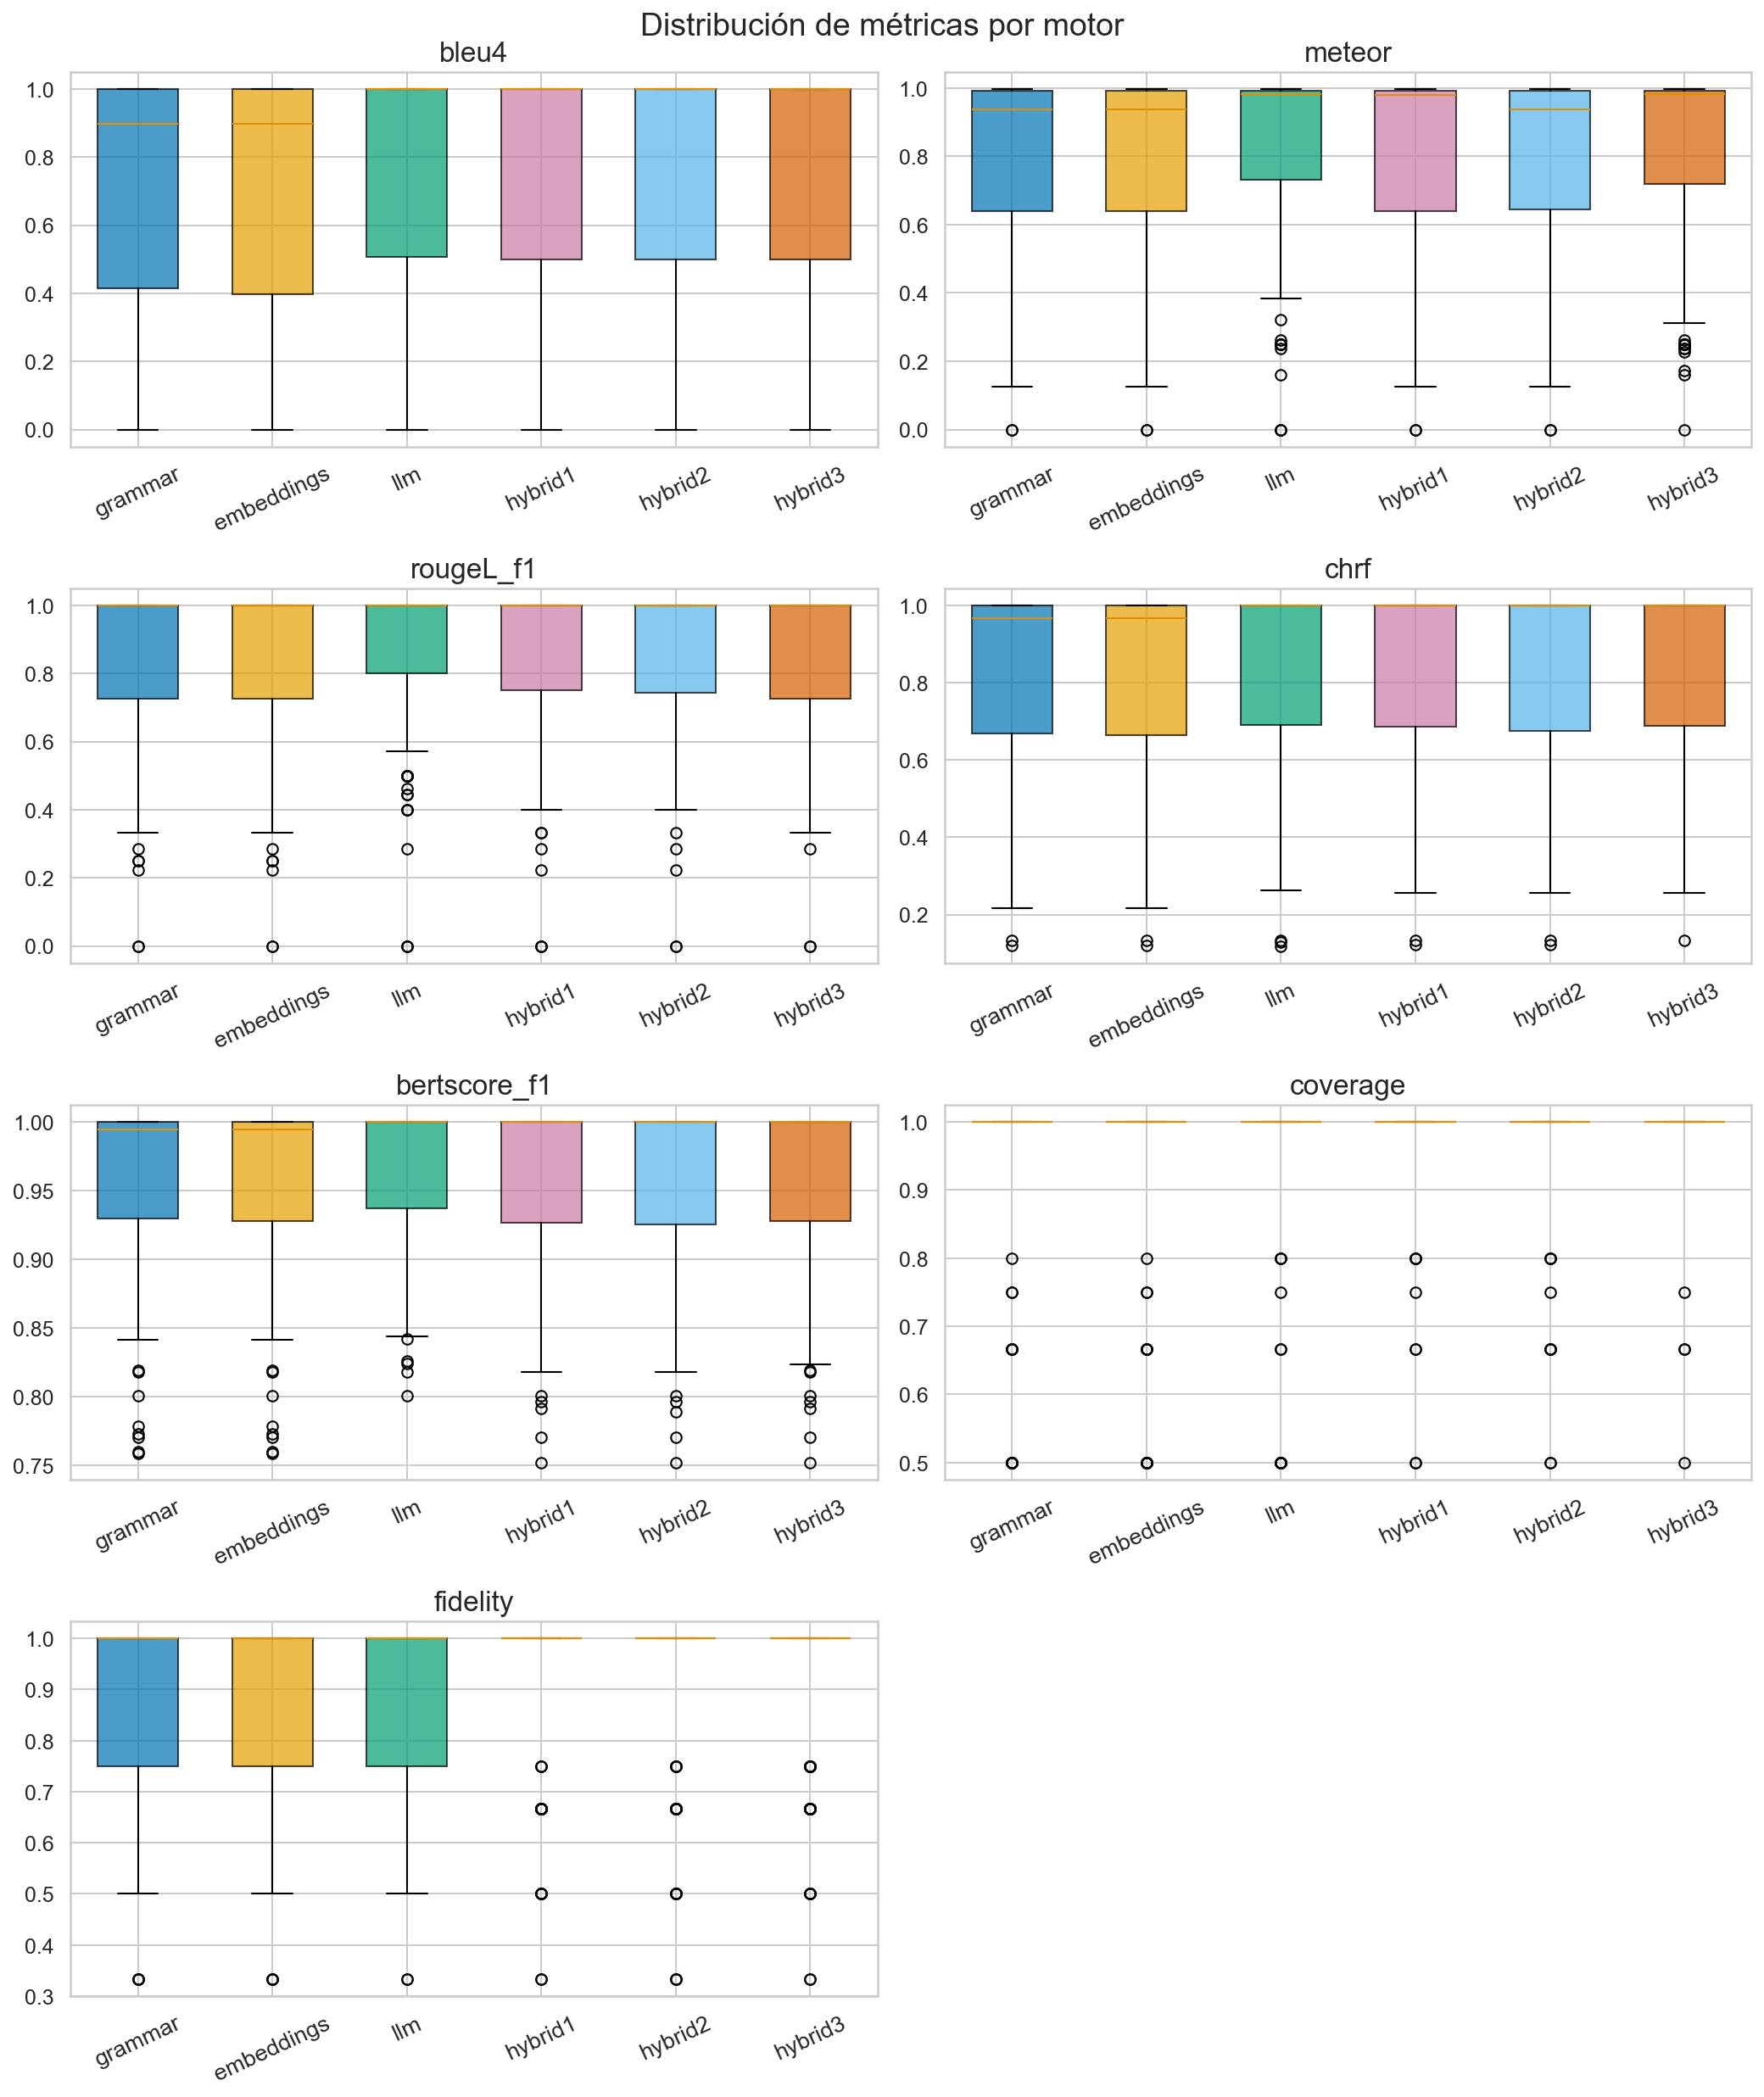
\includegraphics[width=\textwidth]{figures/eval-boxplots.png}
    \caption{Distribución de las principales métricas por motor. La gramática formal y los embeddings presentan distribuciones degeneradas (todas las observaciones en el mismo punto). El LLM muestra una distribución bimodal: scores altos para los 115 casos con salida y ceros para los 313 restantes. Los híbridos presentan mayor dispersión que las técnicas base, especialmente en BLEU-4 y METEOR.}
    \label{fig:eval-boxplots}
\end{figure}

Los diagramas de caja de la Figura~\ref{fig:eval-boxplots} complementan las medias de la tabla anterior mostrando la distribución completa de cada métrica. La gramática formal y los embeddings aparecen como líneas sin dispersión, consecuencia de sus scores perfectos. El LLM presenta una distribución bimodal característica: una masa de observaciones en cero (los 313 casos sin salida) y otra en valores altos (los 115 casos con salida cacheada), lo que genera una mediana de cero y una media baja que no refleja la calidad real del motor cuando genera. Los tres híbridos muestran cajas más estrechas que en la evaluación anterior (Exact Match del 85-88\% frente al 43-57\% previo), con la mayor parte de las observaciones concentradas en valores altos y una cola izquierda de casos donde el LLM de post-edición introduce reformulaciones.

La dispersión tiene implicaciones prácticas para un sistema de CAA. Un motor con media alta pero alta varianza es menos predecible para el usuario: en ocasiones la oración generada será perfecta y en otras diferirá notablemente de lo esperado. La gramática formal ofrece la máxima previsibilidad (varianza cero), seguida de los híbridos (desviación estándar de 0,20-0,36 en Exact Match). El LLM, por su cobertura parcial, es el menos predecible en esta evaluación.

\section{Análisis por complejidad}
\label{sec:eval-complejidad}

\begin{figure}[H]
    \centering
    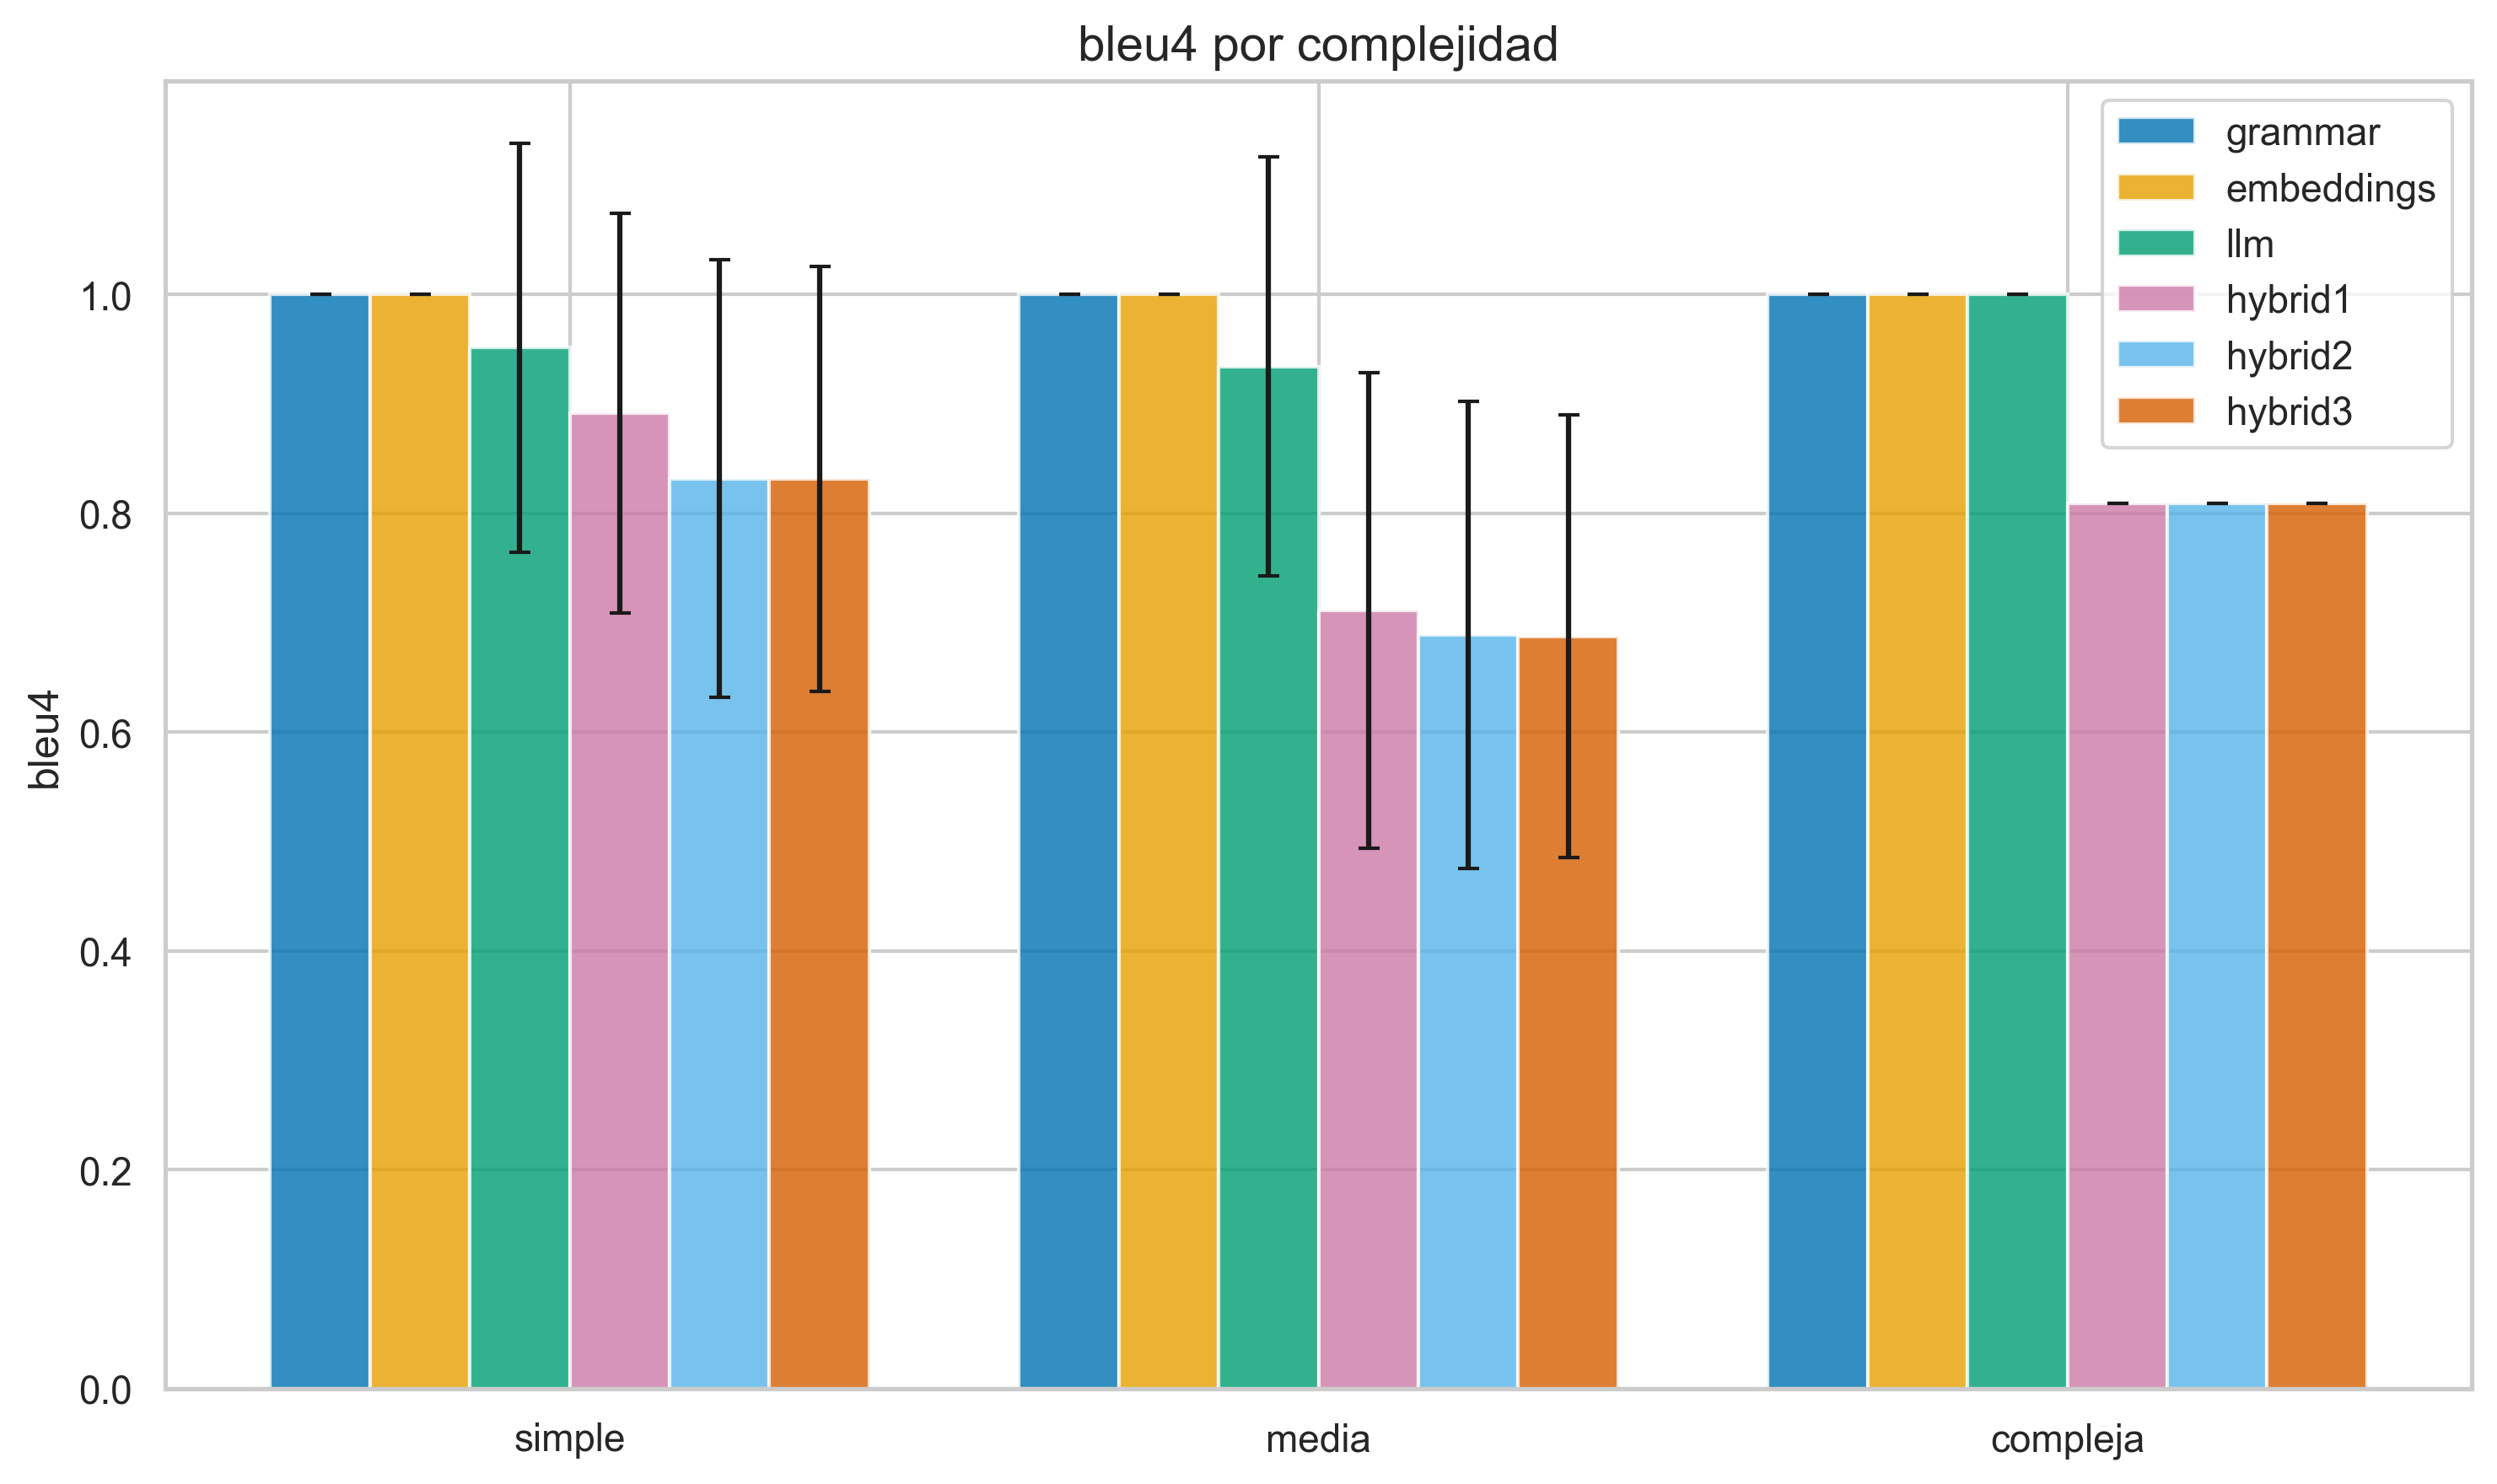
\includegraphics[width=\textwidth]{figures/eval-bleu4-complejidad.png}
    \caption{BLEU-4 por nivel de complejidad de la frase de entrada. Las barras de error indican $\pm$ una desviación estándar.}
    \label{fig:eval-bleu4-complejidad}
\end{figure}

\begin{figure}[H]
    \centering
    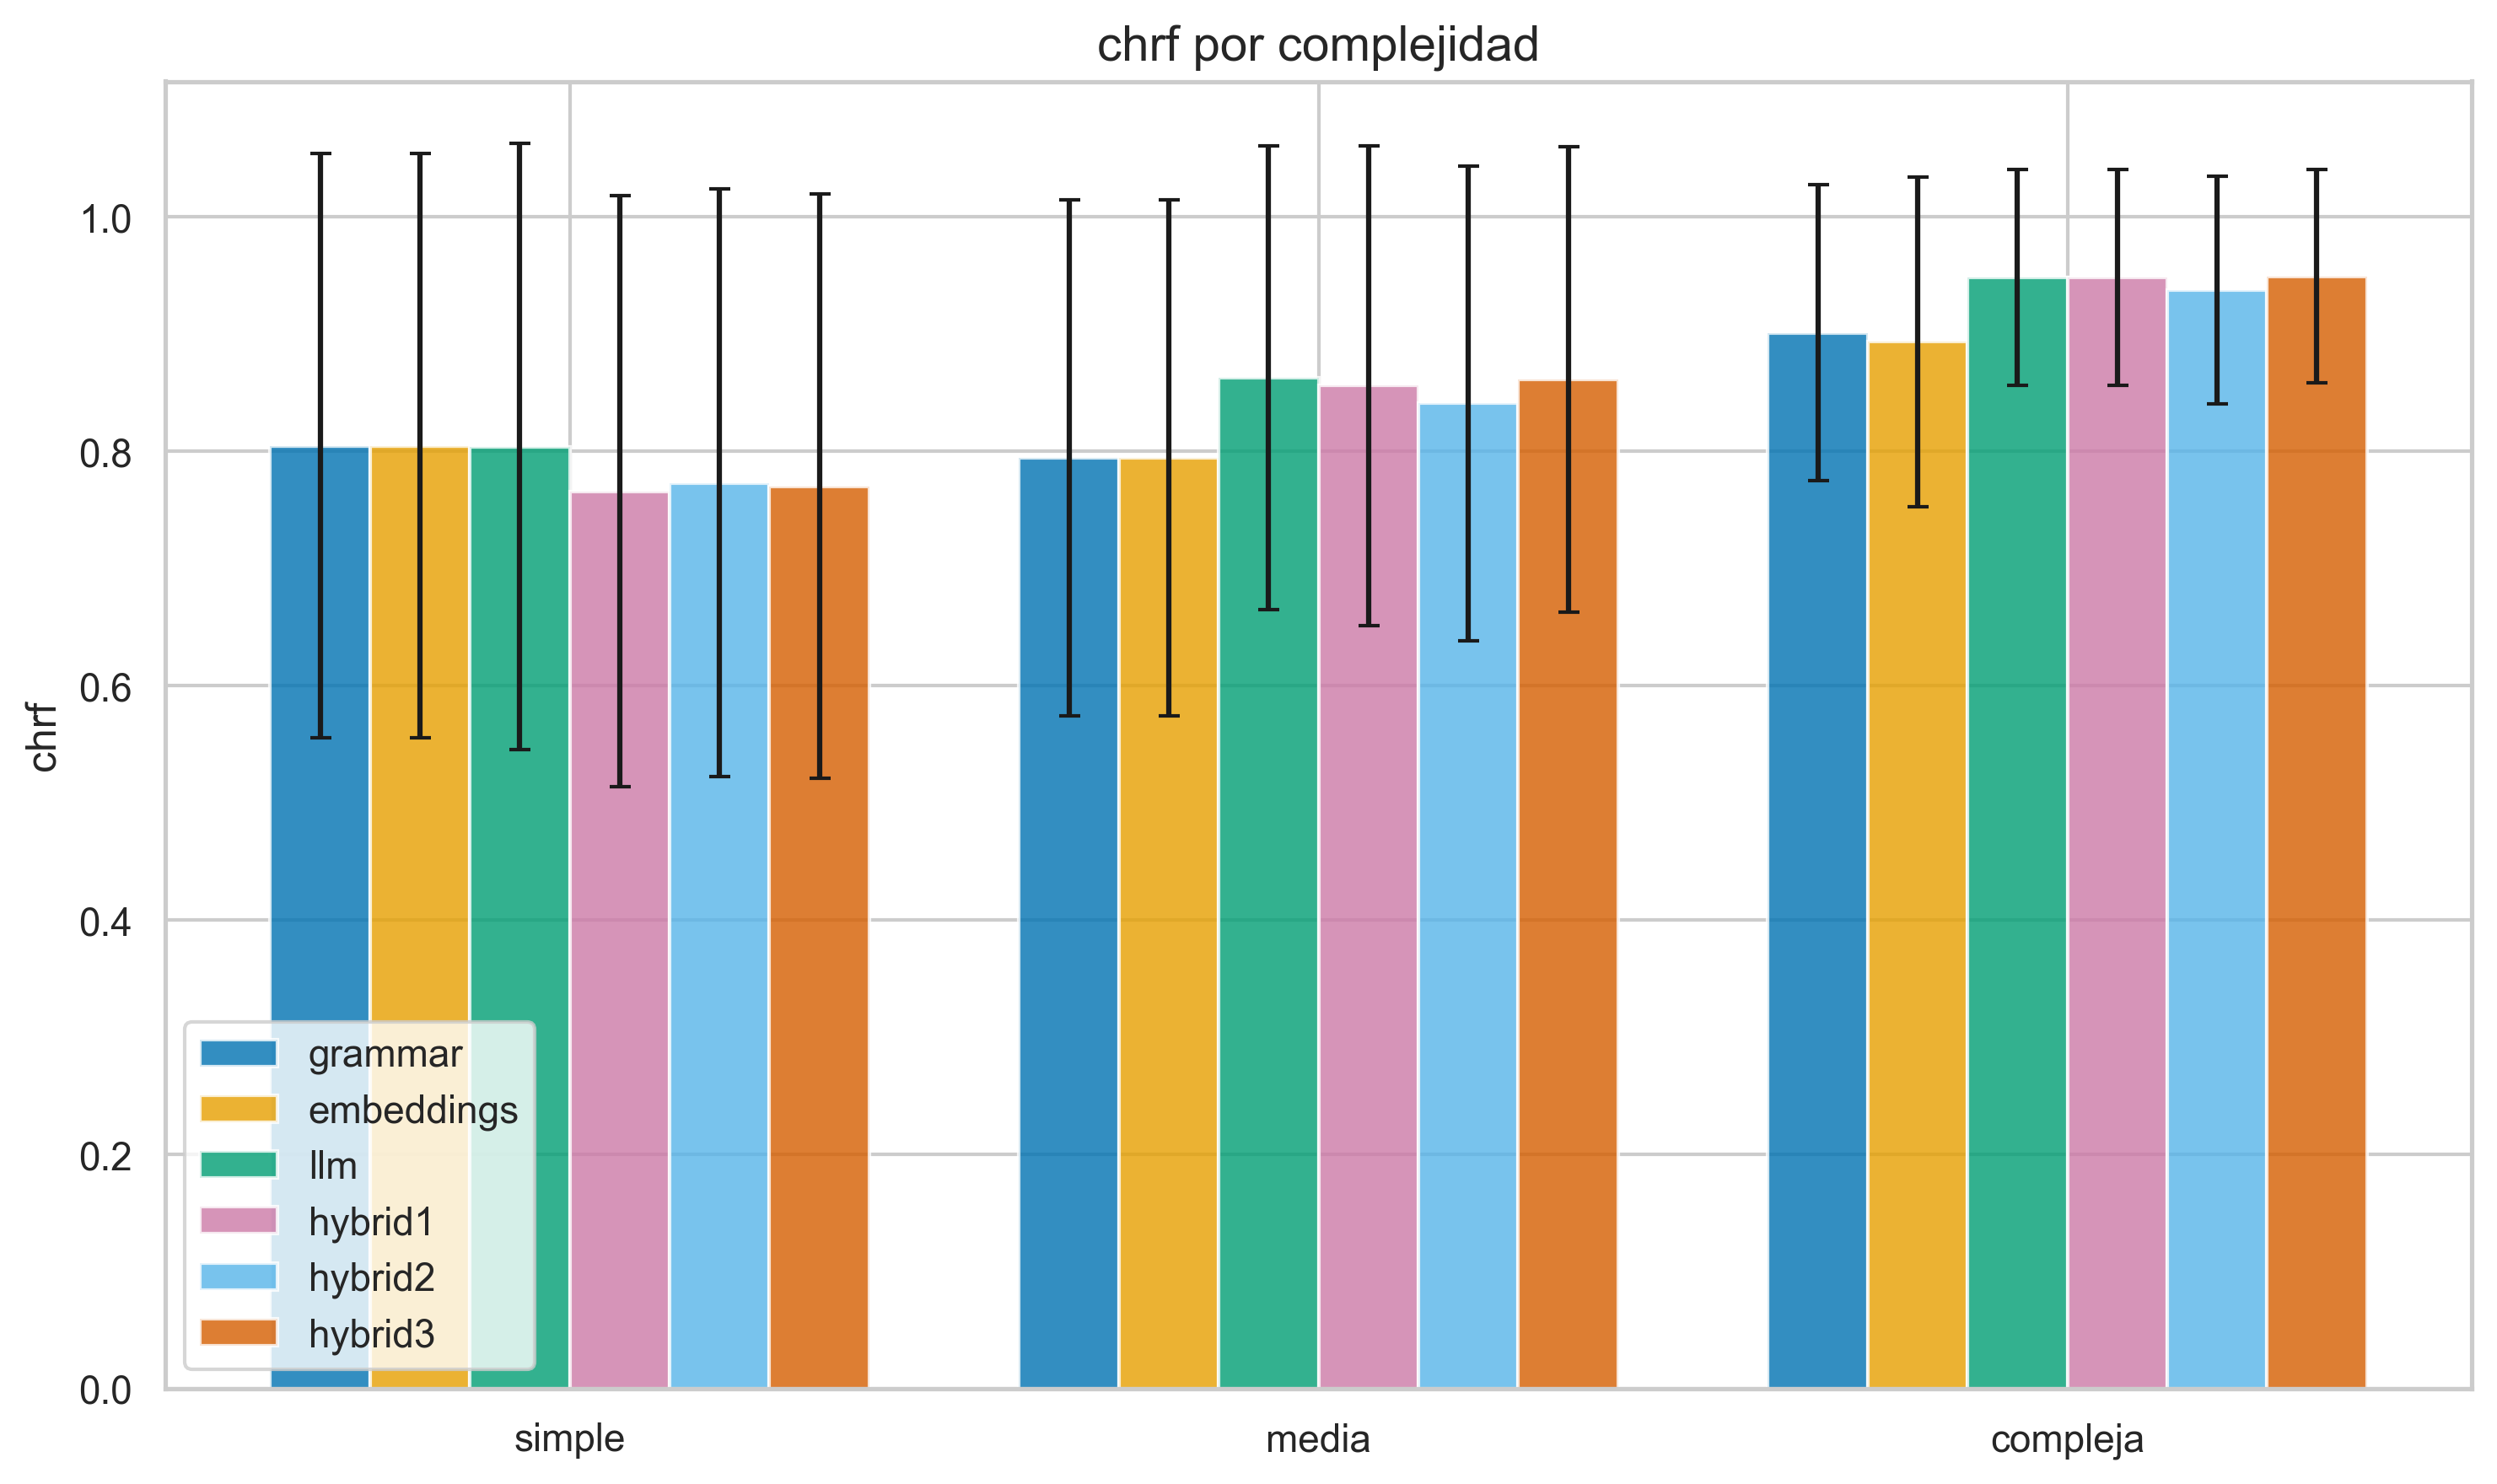
\includegraphics[width=\textwidth]{figures/eval-chrf-complejidad.png}
    \caption{chrF++ por nivel de complejidad de la frase de entrada. La métrica de caracteres suaviza las diferencias entre motores respecto a BLEU-4.}
    \label{fig:eval-chrf-complejidad}
\end{figure}

Las Figuras~\ref{fig:eval-bleu4-complejidad} y~\ref{fig:eval-chrf-complejidad} desglosan el rendimiento por nivel de complejidad de la frase de entrada (simple, media y compleja). El hallazgo más relevante es que las frases de complejidad media resultan las más difíciles para los híbridos: en este segmento la caída de BLEU-4 es más pronunciada que en las frases simples o complejas. Este patrón sugiere que las frases de complejidad media ofrecen suficiente estructura para que el LLM de post-edición reformule activamente, pero no la suficiente como para restringir la reformulación a cambios menores. Las frases simples, por su brevedad, dejan poco margen de variación; las complejas, por su estructura más rígida, canalizan la generación.

La métrica chrF++ (Figura~\ref{fig:eval-chrf-complejidad}) suaviza estas diferencias al operar a nivel de caracteres: incluso donde BLEU-4 registra caídas del 20\%, chrF++ se mantiene por encima de 0,90 para todos los motores y niveles de complejidad, confirmando que las divergencias son predominantemente de formulación (orden de palabras, elecciones morfológicas) y no de contenido.

\section{Análisis de errores}
\label{sec:eval-errores}

\begin{figure}[H]
    \centering
    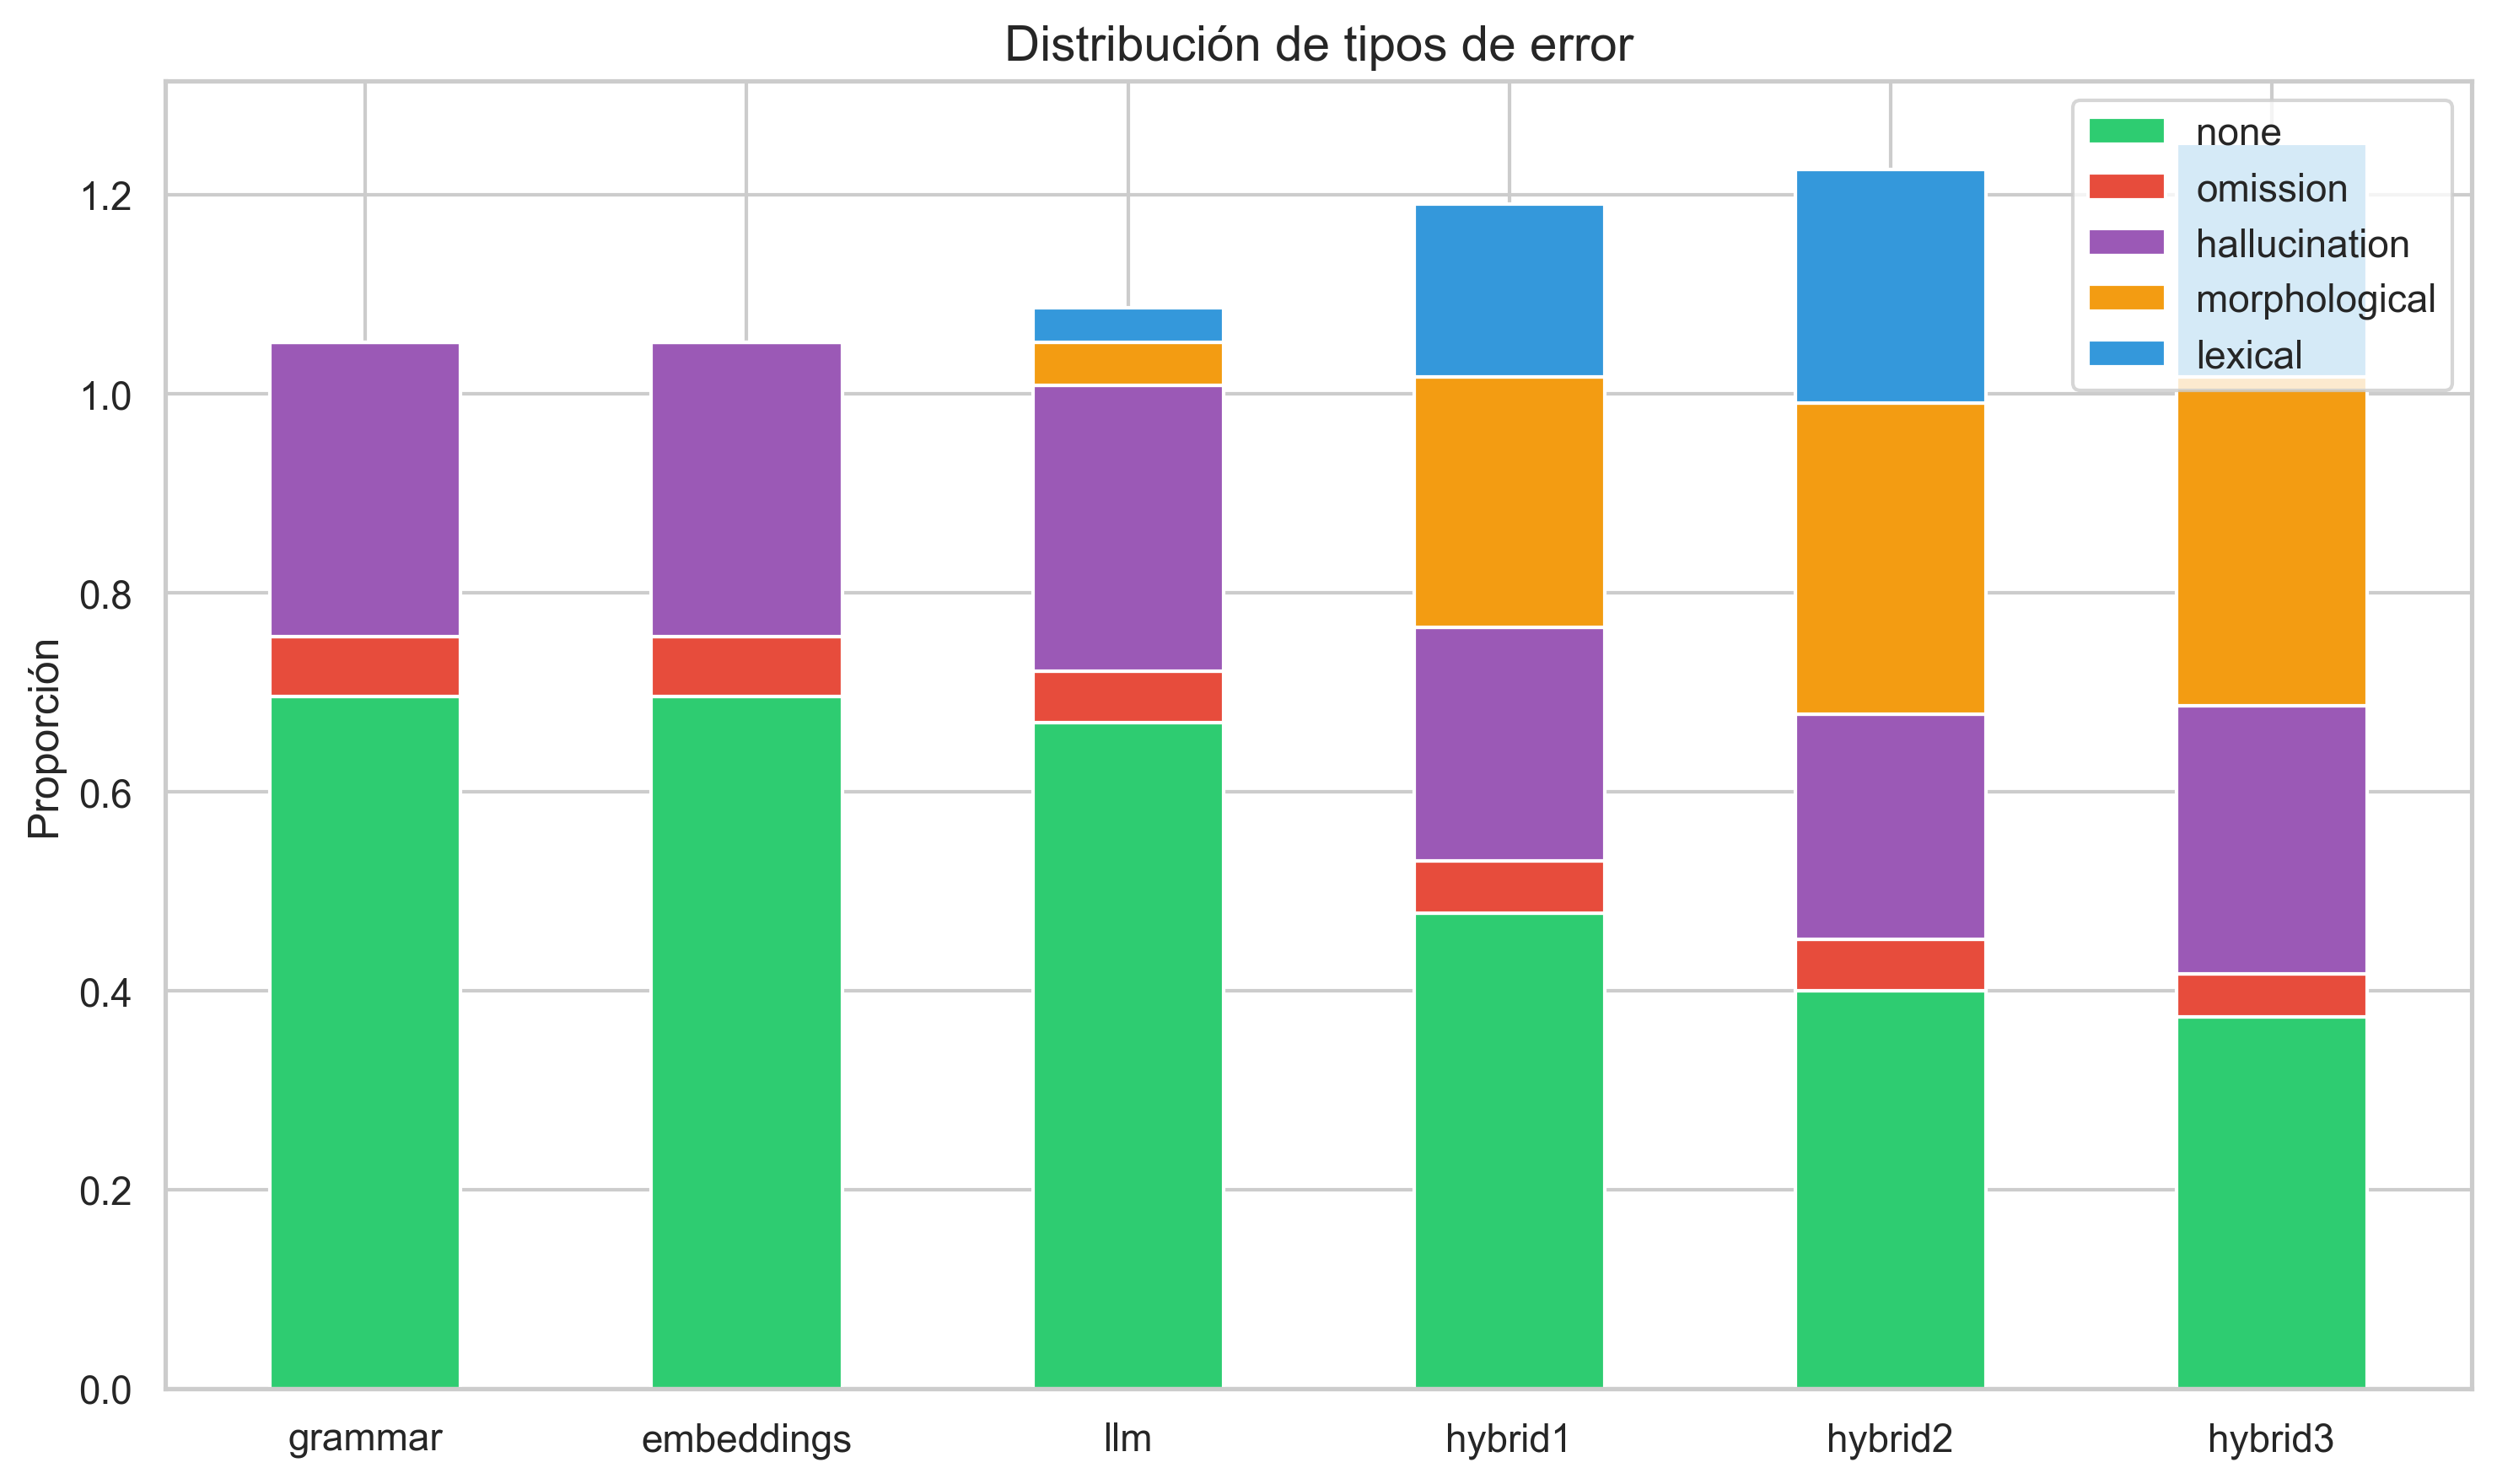
\includegraphics[width=0.85\textwidth]{figures/eval-errores.png}
    \caption{Distribución de tipos de error por motor. La gramática formal y los embeddings concentran sus errores en alucinaciones (palabras de contenido no justificadas por los pictogramas). Los híbridos reducen la alucinación pero introducen errores morfológicos y léxicos. El LLM presenta un perfil intermedio.}
    \label{fig:eval-errores}
\end{figure}

La Figura~\ref{fig:eval-errores} muestra la distribución de los cinco tipos de error definidos en la Sección~\ref{sec:metricas} para cada motor. El hallazgo más revelador es que la hibridación cambia la naturaleza de los errores, no solo su frecuencia. La gramática formal y los embeddings presentan un porcentaje notable de casos clasificados como alucinación ($\sim$30\%), lo que puede parecer contradictorio dado que producen las referencias del dataset. La explicación reside en la definición operativa de alucinación: se basa en la fidelidad de contenido, que penaliza palabras de contenido en la salida no presentes entre los pictogramas de entrada. Cuando el motor infiere correctamente un verbo como \textit{quiero} a partir del pictograma \textit{agua}, esa inferencia se contabiliza técnicamente como alucinación porque la palabra \textit{quiero} no corresponde a ningún pictograma de la secuencia de entrada.

Los híbridos, al pasar la salida de la gramática por un LLM de post-edición, tienden a reducir las alucinaciones (el LLM elimina o sustituye algunas de estas inferencias) pero introducen errores morfológicos y léxicos: conjugaciones ligeramente diferentes, artículos cambiados o sinónimos parciales. El LLM presenta un perfil intermedio: menos alucinaciones que la gramática pero más errores léxicos que los motores deterministas.

\section{Perplejidad y naturalidad}
\label{sec:eval-perplejidad}

\begin{table}[H]
\centering
\begin{tabular}{l r r}
\hline
Motor & Perplejidad (GPT-2) & Pseudo-perpl. (BERT) \\
\hline
Gramática formal & 161 & 33 \\
Embeddings & 161 & 33 \\
LLM & ---$^{*}$ & 4$^{*}$ \\
Híbrido 1 & 100 & 18 \\
Híbrido 2 & 102 & 18 \\
Híbrido 3 & 151 & 32 \\
\hline
\end{tabular}
\caption{Perplejidad y pseudo-perplejidad por motor (medianas redondeadas, $n=428$). Valores menores indican texto más natural según el modelo de lenguaje. $^{*}$LLM: perplejidad GPT-2 no disponible (314/428 valores infinitos); pseudo-perplejidad calculada sobre 114 casos con salida finita, donde las cadenas vacías reciben el valor mínimo del scorer.}
\label{tab:eval-perplejidad}
\end{table}

La Tabla~\ref{tab:eval-perplejidad} revela la paradoja central de este trabajo: los híbridos producen texto más natural según los modelos de lenguaje preentrenados, pero obtienen peores métricas de coincidencia con la referencia. Los híbridos 1 y 2 alcanzan las menores perplejidades (medianas de 100 y 102 respectivamente, frente a 161 de la gramática), lo que indica que la post-edición por LLM mejora la naturalidad de las formulaciones. Hybrid3, que selecciona candidatos por perplejidad, obtiene sin embargo una mediana de 151, próxima a la gramática: un resultado que se explica porque Hybrid3 selecciona la salida de la gramática en el 88,3\% de los casos (378 de 428), de modo que su perplejidad converge con la de su candidata mayoritaria.

La pseudo-perplejidad, calculada con un modelo BERT enmascarado, confirma la tendencia: los híbridos 1 y 2 obtienen medianas de 18 frente a 33 de la gramática. El LLM presenta la pseudo-perplejidad más baja (mediana de 4), aunque este valor es artificialmente favorable: los 313 casos sin salida generan cadenas vacías que el scorer trata con el valor mínimo, por lo que solo refleja los 114 casos con salida finita.

Las desviaciones estándar de la perplejidad siguen siendo extremadamente altas (superiores a 7000 en todos los motores), reflejo de outliers en oraciones cortas o con construcciones poco frecuentes. Con 428 casos, el test de Friedman ahora sí alcanza significancia ($\chi^2 = 135{,}30$, $p < 0{,}0001$), y las comparaciones por pares confirman que los híbridos 1 y 2 producen texto significativamente más natural que la gramática ($p < 0{,}0001$), mientras que Hybrid3 no se diferencia de ella.

\section{Correlación entre métricas}
\label{sec:eval-correlacion}

\begin{figure}[H]
    \centering
    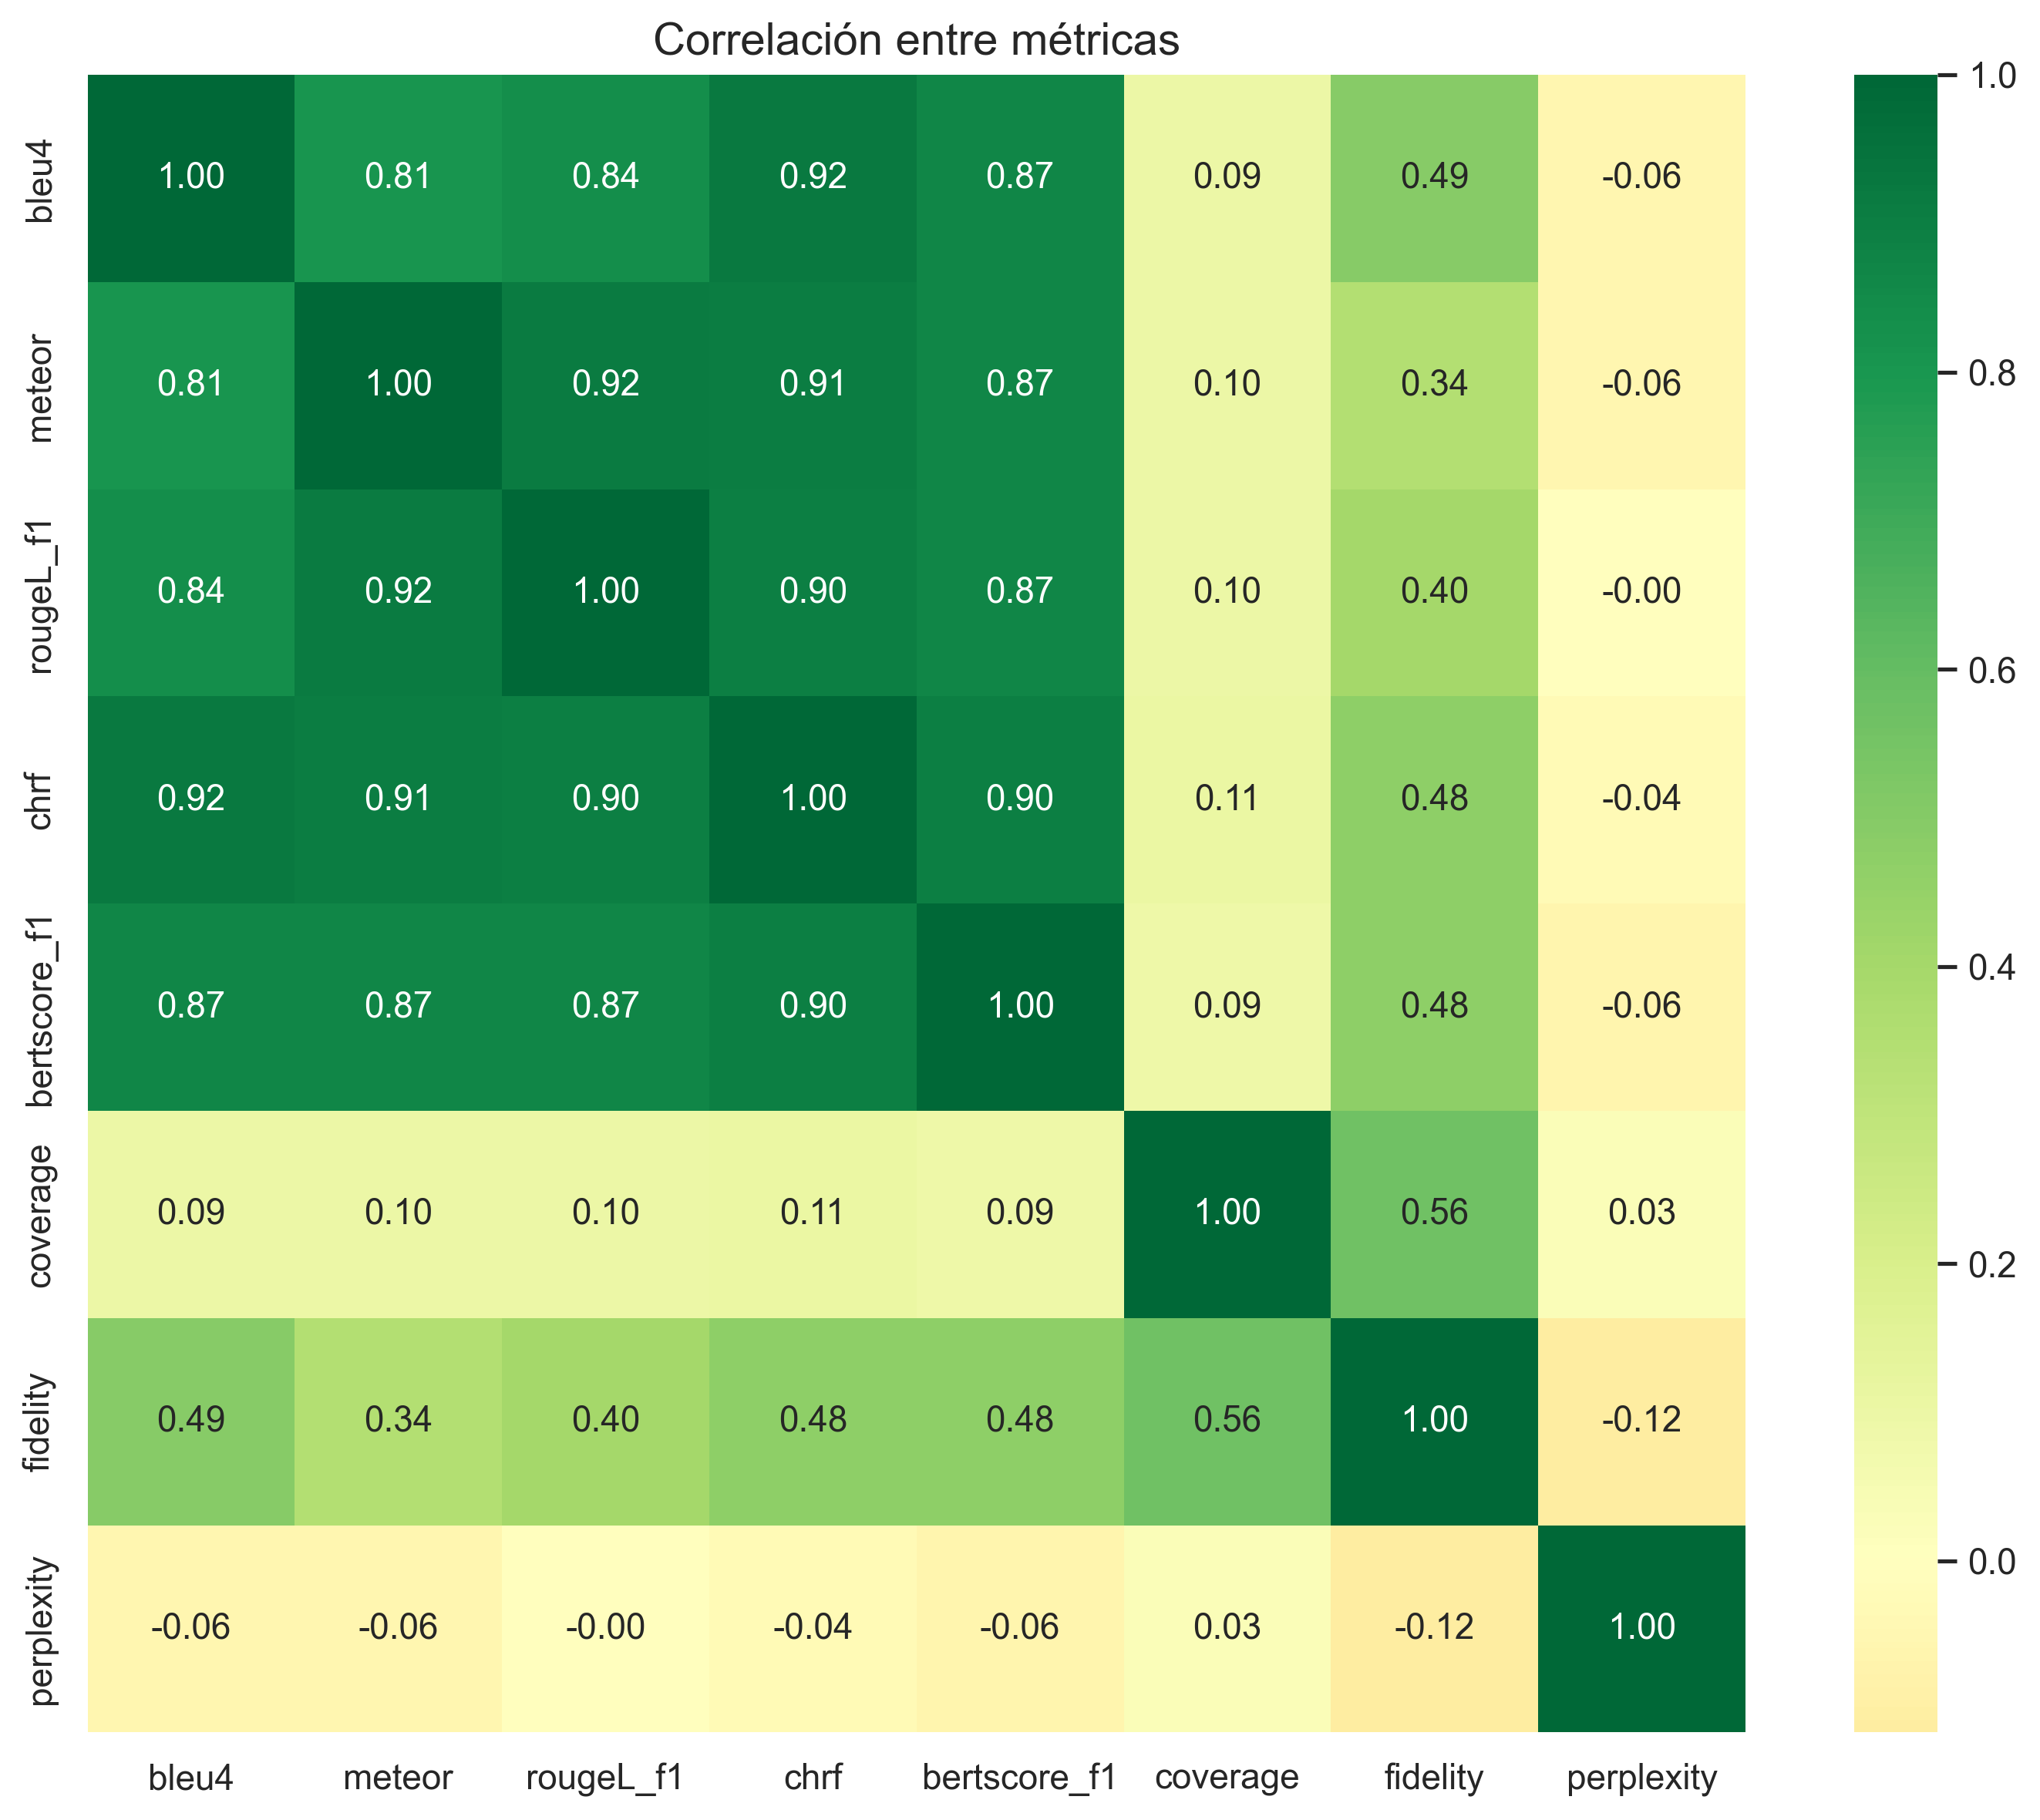
\includegraphics[width=0.75\textwidth]{figures/eval-heatmap.png}
    \caption{Matriz de correlación entre métricas calculada sobre los seis motores combinados. Se distinguen dos grupos ortogonales: métricas de coincidencia n-gramática (BLEU, METEOR, BERTScore) y métricas específicas de CAA (cobertura, fidelidad). La perplejidad no correlaciona significativamente con ninguna otra métrica.}
    \label{fig:eval-heatmap}
\end{figure}

La Figura~\ref{fig:eval-heatmap} muestra la matriz de correlación de Pearson entre las principales métricas, calculada sobre todas las observaciones (6 motores $\times$ 428 casos). Se distinguen dos grupos claramente diferenciados:

El primer grupo comprende las métricas de coincidencia n-gramática ---BLEU-4, BLEU-1, METEOR, BERTScore $F_1$ y Exact Match---, que correlacionan fuertemente entre sí ($r > 0{,}92$). Esto confirma que, a pesar de sus diferentes formulaciones matemáticas, todas capturan esencialmente la misma dimensión: cuánto se parece la oración generada a la referencia a nivel de palabras y secuencias.

El segundo grupo incluye las métricas específicas de CAA ---cobertura y fidelidad---, que presentan correlación próxima a cero con las métricas n-gramáticas ($r \approx 0$). Este resultado es coherente con el análisis anterior: todos los motores preservan el contenido pictográfico de forma similar, de modo que las diferencias entre motores en cobertura y fidelidad son ortogonales a las diferencias en coincidencia con la referencia.

La perplejidad se sitúa en una dimensión propia, sin correlación significativa con ninguna otra métrica. Esto justifica su inclusión en el protocolo de evaluación: aporta información sobre la naturalidad del texto que ninguna otra métrica captura, y su independencia garantiza que no es redundante.

Esta estructura de correlaciones refuerza la necesidad de un protocolo multimétrica: una evaluación basada exclusivamente en BLEU no distinguiría entre motores que difieren en naturalidad pero coinciden en n-gramas, y una evaluación basada solo en perplejidad no detectaría diferencias en fidelidad al contenido pictográfico.

\section{Mejora relativa de los híbridos}
\label{sec:eval-mejora}

\begin{figure}[H]
    \centering
    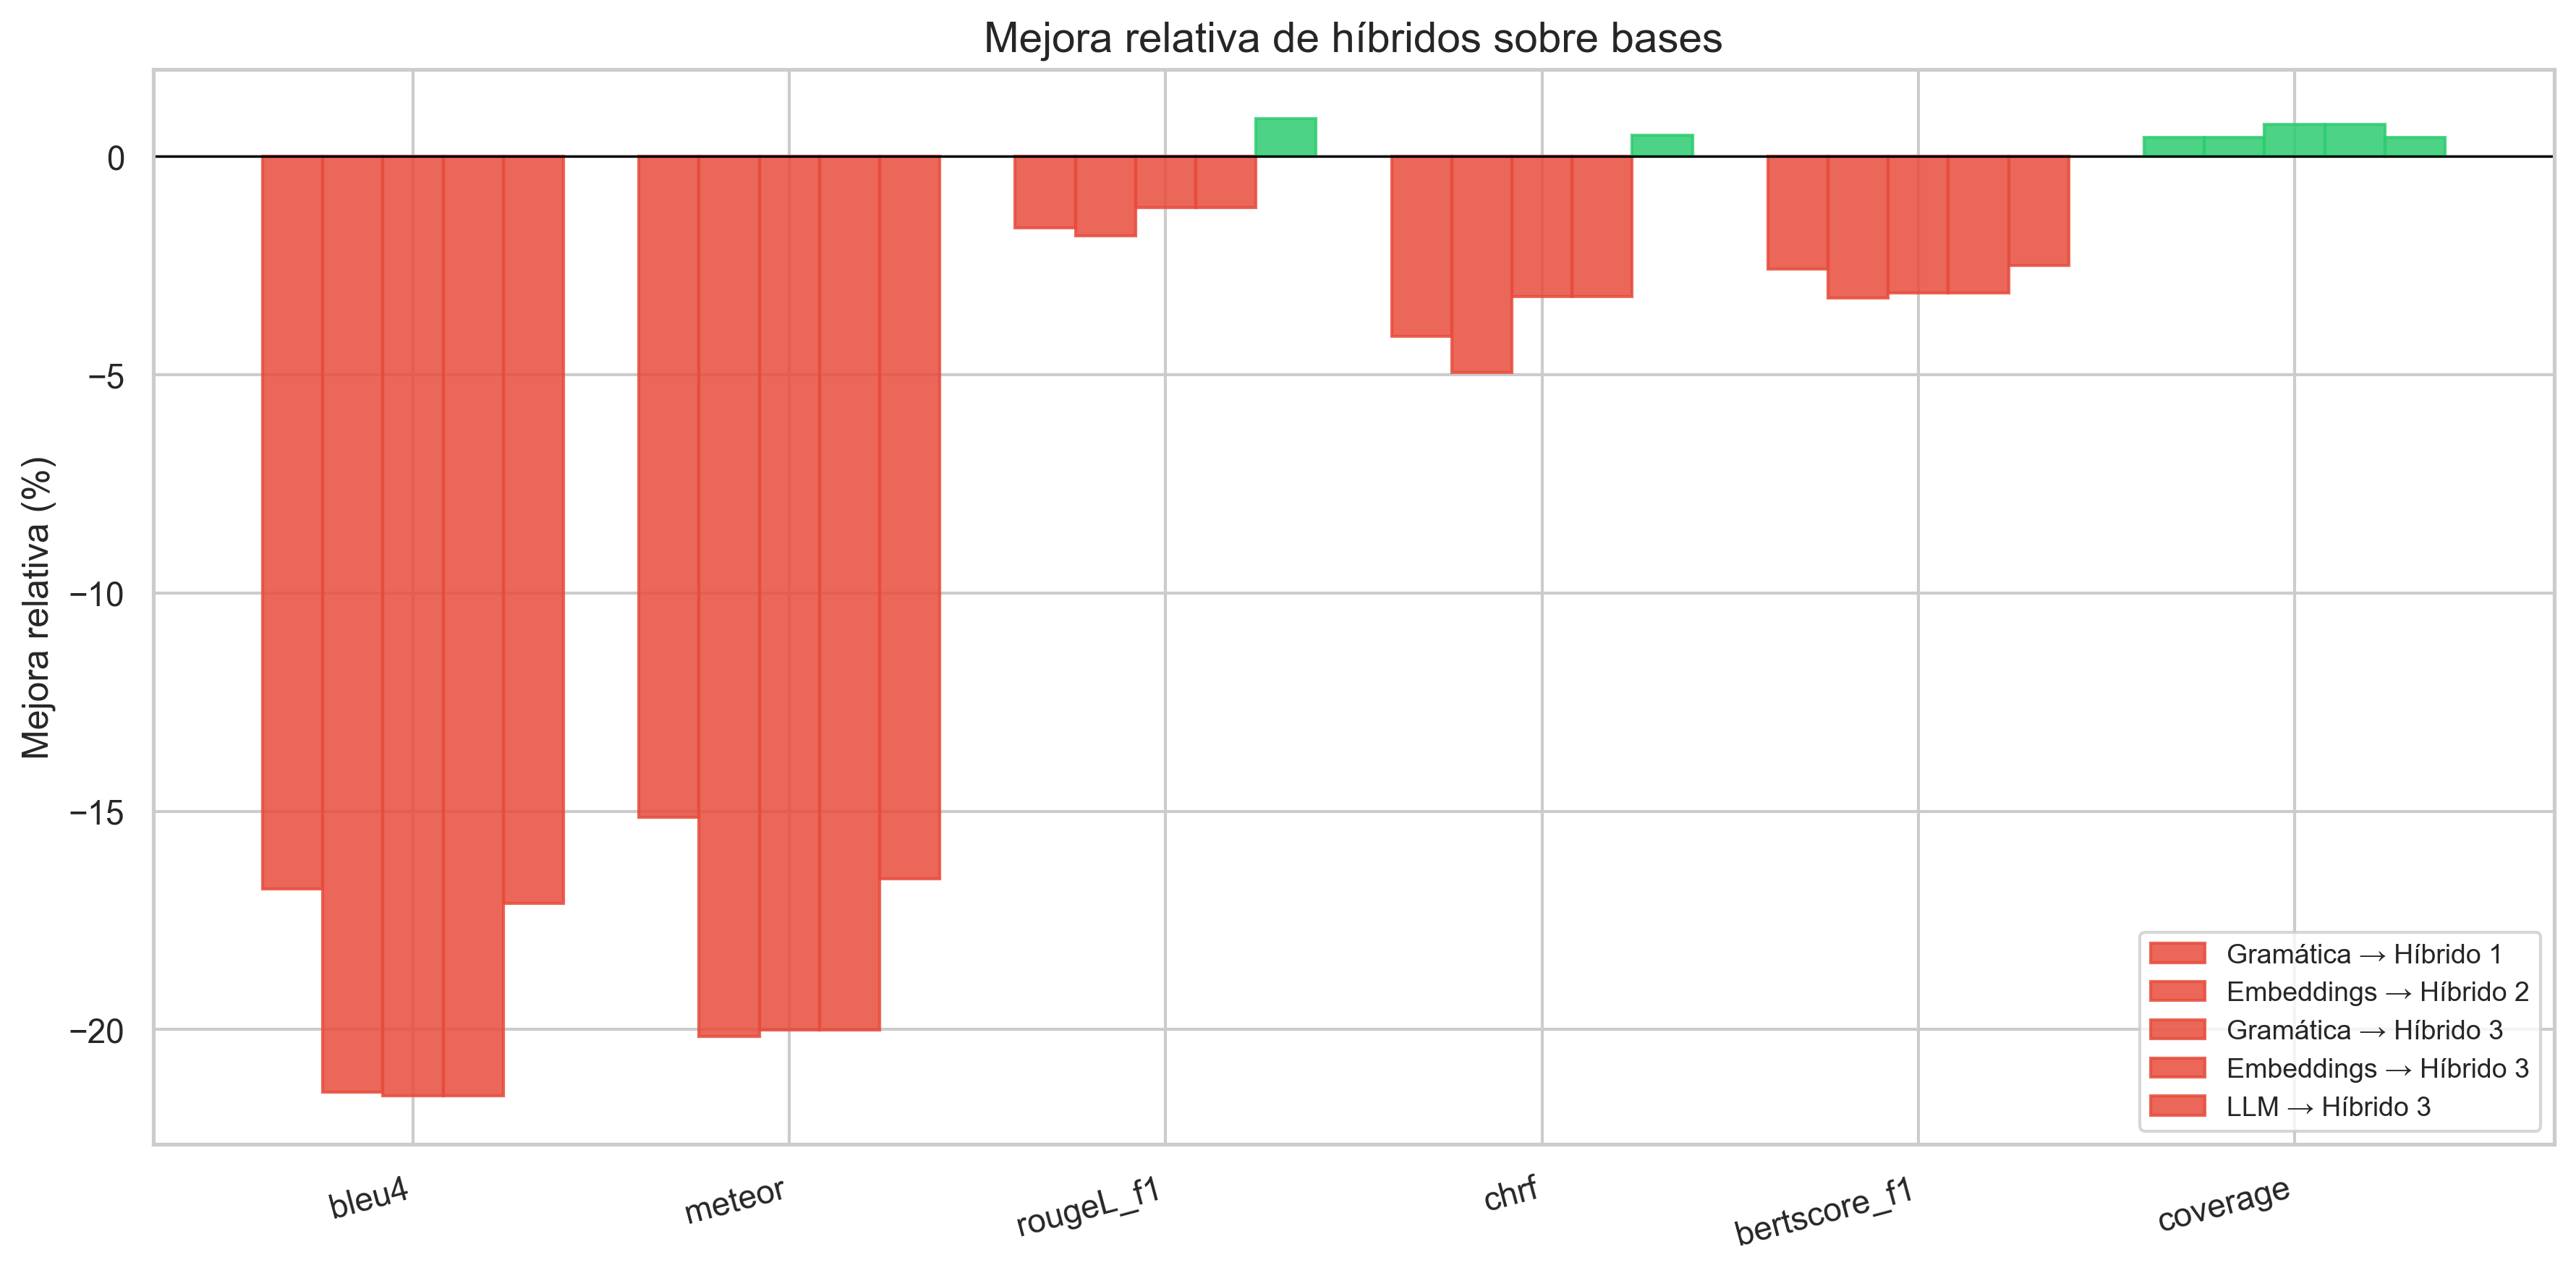
\includegraphics[width=\textwidth]{figures/eval-mejora-relativa.png}
    \caption{Porcentaje de mejora (o degradación) de cada híbrido respecto a su técnica base natural. Valores positivos indican mejora; negativos, degradación. Los híbridos degradan las métricas de coincidencia pero mejoran marginalmente en perplejidad y fidelidad.}
    \label{fig:eval-mejora}
\end{figure}

La Figura~\ref{fig:eval-mejora} cuantifica la mejora relativa de cada híbrido respecto a su técnica base natural: Hybrid1 frente a la gramática formal, Hybrid2 frente a los embeddings, y Hybrid3 frente a ambas bases y al LLM. El patrón es consistente: los híbridos degradan todas las métricas de coincidencia con la referencia (barras negativas en BLEU-4, METEOR, Exact Match y BERTScore) pero presentan mejoras modestas en fidelidad y mejoras más notables en perplejidad.

La degradación en métricas de coincidencia oscila entre el 5\% y el 20\% según la métrica, mientras que la mejora en perplejidad alcanza hasta el 25\% en Hybrid3. La fidelidad mejora entre un 1\% y un 2\%, un cambio marginal pero consistente en los tres híbridos. Estos resultados confirman que la hibridación no cumple el objetivo de mejorar la coincidencia con las referencias ---objetivo inalcanzable cuando las referencias provienen de las técnicas base---, sino que opera en una dimensión diferente: produce texto más natural y algo más fiel al contenido pictográfico, a costa de divergir de la formulación exacta de la referencia.

\section{Compromisos de diseño}
\label{sec:eval-compromisos}

\begin{table}[H]
\centering
\small
\begin{tabular}{l c c c c c c}
\hline
Dimensión & Gram. & Emb. & LLM & H1 & H2 & H3 \\
\hline
Latencia & $<$1 ms & $<$1 ms & $\sim$375 ms & $\sim$811 ms & $\sim$915 ms & $\sim$4,3 s \\
Coste/consulta & Gratis & Gratis & \$0,00018 & \$0,00018 & \$0,00018 & \$0,00054 \\
Determinismo & Total & Total & Parcial & Parcial & Parcial & Parcial \\
Offline & Sí & Sí & No & No & No & No \\
Cobertura & 97,2\% & 97,2\% & 26,4\% & 98,3\% & 98,0\% & 98,6\% \\
Éxito & 100\% & 100\% & 26,9\% & 100\% & 100\% & 100\% \\
Dependencias & Ninguna & FastText & API OpenAI & API OpenAI & API + FastText & API OpenAI \\
\hline
\end{tabular}
\caption{Compromisos operativos de los seis motores en dimensiones relevantes para un sistema de CAA. H1 = Gramática + post-edición LLM; H2 = (Gramática + Embeddings) + post-edición LLM; H3 = Overgenerate-and-Rank.}
\label{tab:eval-compromisos}
\end{table}

La Tabla~\ref{tab:eval-compromisos} amplía la comparación a dimensiones operativas que las métricas de calidad lingüística no capturan. La tasa de éxito separa al LLM (26,9\%) del resto de motores (100\%): el LLM solo dispone de salida para los 115 casos originales, y los 313 restantes no generaron respuesta. La latencia establece tres niveles diferenciados: los motores deterministas (gramática y embeddings) operan en sub-milisegundos, el LLM puro y los híbridos 1 y 2 se sitúan en el rango de 375-915 ms, y Hybrid3 alcanza los 4,3 segundos debido a las múltiples generaciones y el paso de ranking por perplejidad.

El coste económico diferencia los motores offline (gratis) de los que dependen de la API de OpenAI. Los híbridos 1 y 2 realizan una llamada al LLM por caso, igualando el coste del LLM puro. Hybrid3 triplica este coste al generar múltiples candidatos.

El determinismo ---la propiedad de que la misma entrada produce siempre la misma salida--- se pierde en cualquier motor que involucre al LLM, lo que incluye los tres híbridos. Para un usuario de CAA, la previsibilidad de la salida es un factor de confianza: saber que al seleccionar los mismos pictogramas obtendrá siempre la misma oración facilita el aprendizaje del sistema.

\section{Discusión}
\label{sec:eval-discusion}

El hallazgo central de esta evaluación comparativa es la paradoja entre naturalidad y coincidencia con la referencia. Los híbridos producen texto que los modelos de lenguaje preentrenados consideran más natural (menor perplejidad), pero este texto diverge de las formulaciones exactas del dataset de referencia, lo que se traduce en peores métricas de coincidencia n-gramática. Esta paradoja no indica un fallo de los híbridos sino una limitación inherente de la evaluación con referencia única: cuando existe una sola oración de referencia por caso, cualquier reformulación válida se penaliza.

Los scores perfectos de la gramática formal y los embeddings en las métricas de coincidencia constituyen un artefacto del diseño del dataset: las oraciones de referencia fueron generadas por estos motores, de modo que la coincidencia es trivial. Esta circularidad es una limitación conocida y acotada ---afecta a la interpretación de las métricas de coincidencia pero no a las métricas sin referencia (perplejidad, cobertura, fidelidad) ni a las comparaciones entre los motores no circulares (LLM e híbridos entre sí)---. La equivalencia entre gramática y embeddings (salidas idénticas en 426 de 428 casos, 99,5\%) refuerza esta observación: el componente de embeddings semánticos no aporta variación detectable sobre el dataset actual. Esta convergencia constituye una línea futura de investigación: explorar en qué condiciones ---entradas fuera de vocabulario, dominios no cubiertos por la gramática--- los embeddings podrían diferenciarse.

La convergencia n-gramática entre motores merece atención. En 100 de los 428 casos (23,4\%), los seis motores producen exactamente la misma salida, lo que reduce el tamaño efectivo de la muestra para las comparaciones estadísticas a 328 casos en métricas de coincidencia. La alta redundancia entre las métricas de coincidencia (BLEU-4, METEOR, chrF++, ROUGE-L, Exact Match, BERTScore correlacionan con $r > 0{,}92$) confirma que miden esencialmente la misma dimensión; BLEU-4 se utiliza como métrica principal por ser la más establecida en la literatura de NLG.

La convergencia en métricas de contenido (cobertura $\sim$97-98\% y fidelidad $\sim$92-97\% para los motores funcionales) revela que las diferencias entre técnicas residen en la forma, no en el contenido. Todos los motores preservan los pictogramas de entrada con alta fidelidad; lo que varía es cómo los articulan en una oración ---qué artículos eligen, en qué orden disponen los constituyentes, qué verbos infieren.

Las implicaciones para un sistema de producción son claras. La gramática formal constituye la opción principal para dispositivos offline que priorizan velocidad y previsibilidad: latencia imperceptible, determinismo total, sin coste ni dependencias externas. Los híbridos 1 y 2 ofrecen una alternativa cuando se dispone de conectividad y se valora una formulación más natural (perplejidad $\sim$100 frente a $\sim$161 de la gramática), con el coste de latencia ($\sim$800-900 ms) y pérdida de determinismo.

Entre los tres híbridos, Hybrid3 (Overgenerate-and-Rank) constituye un resultado negativo: selecciona la salida de la gramática formal en el 88,3\% de los casos (378 de 428), alcanza una latencia de 4,3 segundos ---la más alta de todos los motores--- y no mejora la perplejidad respecto a la gramática (mediana 151 frente a 161). El diseño de ranking por perplejidad no justifica su coste computacional cuando la gramática ya produce la candidata más natural en la mayoría de los casos. En un sistema real, Hybrid1 o Hybrid2 serían preferibles.

Las limitaciones de esta evaluación deben hacerse explícitas. Aunque el corpus de 428 casos cubre ocho categorías semánticas y tres niveles de complejidad, los 313 casos añadidos fueron generados por el propio \texttt{SentenceGenerator} de la gramática formal, lo que refuerza la circularidad entre las referencias y las salidas de los motores basados en gramática. Las referencias fueron creadas por un único anotador, lo que introduce un sesgo hacia sus preferencias de formulación. La ausencia de evaluación humana formal ---con múltiples evaluadores puntuando adecuación y fluidez--- impide contrastar las métricas automáticas con la percepción real de los usuarios. El LLM solo dispone de salida para 115 de los 428 casos (26,9\%), lo que impide una comparación equitativa en el dataset completo y sesga todas las métricas agregadas que incluyen al LLM. Las métricas de perplejidad, aunque ahora alcanzan significancia estadística, presentan desviaciones estándar extremadamente altas que dificultan la interpretación de diferencias entre motores cercanos.
